\newcommand{\Author}{Simon Symhoven}
\newcommand{\Strasse}{Boschetsriederstra\ss{}e 59a}
\newcommand{\Stadt}{D-81379 M\"unchen}
\newcommand{\Email}{simon.symhoven@hm.edu}
\newcommand{\Matrikelnummer}{49651418}
\newcommand{\Fachsemester}{6}
\newcommand{\Studiengang}{Wirtschaftsinformatik}
\newcommand{\TitelArbeit}{Ein konfigurierbares und skalierbares Monitoringsystem f\"ur Delta-Metriken innerhalb des kontinuierlichen Integrationsservers Jenkins}
\newcommand{\UntertitelArbeit}{Untertitel}
\newcommand{\Labor}{Bachelor - Thesis}
\newcommand{\Prof}{Prof. Dr. Ullrich Hafner}
\newcommand{\Semester}{Sommersemester 2021}
\newcommand{\Fachbereich}{Informatik und Mathematik}
\newcommand{\Datum}{\today}
\newcommand{\HRule}{\rule{\linewidth}{0.3mm}}

\makeglossary


%
% Einbinden des Headers, hier können auch weitere Einstellungen vorgenommen werden.
%%%%%%%%%%%%%%%%%%%%%%%%%%%%%%%%%%%%%%%%%%%%%%%%%%%%%%%
%																					%
%	In dieser Datei werden alle Packages eingebunden, 	%
% welche für das Dokument nötig sind. Desweiteren 		%
% werden die Dokumentinformationen gesetzt.						%
%																											%
%%%%%%%%%%%%%%%%%%%%%%%%%%%%%%%%%%%%%%%%%%%%%%%%%%%%%%%
%
%	Die KOMAScript Dokumentklasse "scrbook" verwenden.
%
\documentclass[pdftex, 		%
							a4paper, 		% DIN A4 verwenden
							titlepage,	% separate Titelseite
							%draft,			%	Draft-Version, keine Bilder im pdf!
							final,			% Final-Version
							oneside,		% einseitiger Druck
							11pt,				% Schriftgröße 12pt
							DIV=calc,
							%tocbasic,
							]{scrbook}	%	KOMAScript scrbook-Dokumentklasse
							
%%%%%%%%%%%%%%%%%%%%%%%%%%%%%%%%%%%%%%%%%%%%%%%%%%%%%%%%
%	Einbinden der Pakete 
%%%%%%%%%%%%%%%%%%%%%%%%%%%%%%%%%%%%%%%%%%%%%%%%%%%%%%%%

\usepackage{tabularx}

\usepackage{afterpage}

\newcommand\blankpage{%
    \null
    \thispagestyle{empty}%
    \addtocounter{page}{-1}%
    \newpage}
    
% PDF Dateien einbinden
\usepackage{pdfpages}
\usepackage{float}
%Settings for PDF Pages to accept additonal versioned PDF files
\pdfminorversion=6
\pdfcompresslevel=9
\pdfobjcompresslevel=9

%Infos dazu unter: http://www.bakoma-tex.com/doc/latex/koma-script/scrhack.pdf
%Einige Pakete haben Probleme mit dem Komaskript.
\usepackage{scrhack} 

% Abkürzungsverzeichnis
\usepackage{acronym}

% Definieren von eigenen benannten Farben.
% Für spätere Verwendung in dem Dokument, definieren wir einzelne
% benannte Farben.
%
\usepackage{xcolor}
\definecolor{gray1}{gray}{0.92}
\definecolor{darkgreen}{rgb}{0,0.5,0}

\definecolor{urlLinkColor}{rgb}{0,0,0.5}
\definecolor{LinkColor}{rgb}{0,0,0}
\definecolor{ListingBackground}{rgb}{0.85,0.85,0.85}
\definecolor{hmred}{RGB}{251, 86, 85}

\usepackage[ngerman]{babel}

\rmfamily
\usepackage[numbers, square]{natbib}
		% Schriftfamilie Palatino

%\usepackage[dvips]{color}    	% für graue Boxen
%\usepackage[dvips]{graphicx} 	% Grafikpaket
\usepackage{makeidx}   				% Paket zur Erzeugung eines Index
\usepackage[normalem]{ulem}   % bietet Unterstreichungsvarianten
\usepackage{picins} 					% Bilder im Absatz platzieren
\usepackage[T1]{fontenc}			% Erweiterten Zeichensatz aktivieren
\usepackage{lmodern}
\setlength{\emergencystretch}{1em} 		
\usepackage{multido}					% ermöglicht Schleifenartiges wiederholen von Befehlen
\usepackage{mdwlist}					% ermöglicht das Setzen des Zählers bei Aufzählungspunkten
\usepackage{paralist}					% Paket für Aufzählungen, erweitert Enumerate-Paket
\usepackage{longtable}				% mehrseitige Tabellen
\usepackage{tocbasic}
\parindent0pt           			% verzichte auf Einrücken der ersten Zeile
\parskip1ex             			% Abstand zwischen den Absätzen
\usepackage{setspace}					% Paket zum Einstellen des Zeilenabstands
\onehalfspacing								% anderthalbfacher Zeilenabstand
%\doublespacing								% doppelter Zeilenabstand
%\singlespacing								% einfacher Zeilenabstand

%\usepackage[german]{babel}
\usepackage[german=quotes]{csquotes} %Deutsche Anführungszeichen

\usepackage{color}
\definecolor{LinkColor}{rgb}{0.1,0.1,0.1}
%\definecolor{ListingBackground}{rgb}{0.85,0.85,0.85}
\definecolor{ListingBackground}{rgb}{0.98,0.98,0.98}
\definecolor{gray}{rgb}{0.4,0.4,0.4}
\definecolor{darkblue}{rgb}{0.0,0.0,0.6}
\definecolor{cyan}{rgb}{0.0,0.6,0.6}


%
% Farbeinstellungen für die Links im PDF Dokument.
%
\makeindex

%-----------Paket für absolute Positionierung von Grafiken------------------
\usepackage[absolute]{textpos}
\setlength{\TPHorizModule}{1mm}
\setlength{\TPVertModule}{\TPHorizModule}

%-----------Aufzählungen und Einstellungen für Sourcecode-------------------
%\usepackage[savemem]{listings} %Bei wenig Arbeitsspeicher dies Option [savemem] aktivieren.
\usepackage{listings}
\lstloadlanguages{TeX,XML, Java} % TeX sprache laden, notwendig wegen option 'savemem'
\lstset{%
	language=[LaTeX]TeX,     % Sprache des Quellcodes ist TeX
	numbers=left,            % Zelennummern links
	stepnumber=1,            % Jede Zeile nummerieren.
	numbersep=5pt,           % 5pt Abstand zum Quellcode
	numberstyle=\tiny,       % Zeichengrösse 'tiny' für die Nummern.
	breaklines=true,         % Zeilen umbrechen wenn notwendig.
	breakautoindent=true,    % Nach dem Zeilenumbruch Zeile einrücken.
	postbreak=\space,        % Bei Leerzeichen umbrechen.
	tabsize=2,               % Tabulatorgrösse 2
	basicstyle=\ttfamily\footnotesize, % Nichtproportionale Schrift, klein für den Quellcode
	showspaces=false,        % Leerzeichen nicht anzeigen.
	showstringspaces=false,  % Leerzeichen auch in Strings ('') nicht anzeigen.
	extendedchars=true,      % Alle Zeichen vom Latin1 Zeichensatz anzeigen.
	backgroundcolor=\color{ListingBackground}} % Hintergrundfarbe des Quellcodes setzen.

\definecolor{javared}{rgb}{0.6,0,0} % for strings
\definecolor{javagreen}{rgb}{0.25,0.5,0.35} % comments
\definecolor{javapurple}{rgb}{0.5,0,0.35} % keywords
\definecolor{javadocblue}{rgb}{0.25,0.35,0.75} % javadoc
 
\lstset{language=Java,
	basicstyle=\ttfamily,
	keywordstyle=\color{javapurple}\bfseries,
	stringstyle=\color{javared},
	commentstyle=\color{javagreen},
	morecomment=[s][\color{javadocblue}]{/**}{*/},
	numbers=left,
	numberstyle=\tiny\color{black},
	stepnumber=1,
	numbersep=10pt,
	tabsize=4,
	showspaces=false,
	showstringspaces=true}

\lstset{
  basicstyle=\small\ttfamily,
  columns=fullflexible,
  showstringspaces=false,
  %commentstyle=\color{gray}\upshape
}
%neue Lang definieren, als Bsp.
\lstdefinelanguage{XML-changed}
{
  basicstyle=\footnotesize\ttfamily\bfseries,
  morestring=[b]",
  morestring=[s]{>}{<},
  morecomment=[s]{<?}{?>},
  stringstyle=\color{black},
  identifierstyle=\color{darkblue},
  keywordstyle=\color{cyan},
  morekeywords={xmlns,version,type}% list your attributes here
}

%-----------Caption Package-------------------
\usepackage{caption}
\DeclareCaptionFont{white}{\color{white}}
\DeclareCaptionFormat{listing}{\colorbox[cmyk]{0.43, 0.35, 0.35,0.01}{\parbox{\textwidth}{\hspace{15pt}#1#2#3}}}

\DeclareCaptionFormat{graphics}{\colorbox[cmyk]{0.43, 0.35, 0.35,0.01}{\parbox{\textwidth}{\hspace{15pt}#1#2#3}}}


\captionsetup[lstlisting]{format=listing,labelfont=white,textfont=white, singlelinecheck=false, margin=0pt, font={footnotesize}}

%-----------Header+Footer---------------------------------------------------
\usepackage{fancyhdr}					%
\pagestyle{fancy}							%

\fancyhead{}
\fancyfoot{} 
\renewcommand{\headrulewidth}{0.4pt} % Kopzeilenlinie
\renewcommand{\footrulewidth}{0.0pt} % Fusszeilenlinie 0.0pt blendet sie aus

\renewcommand{\chaptermark}[1]{\markboth{\thechapter\quad#1}{}}
\renewcommand{\sectionmark}[1]{\markright{\thesection\quad#1}}

\fancyhead[LO]{\small\sffamily\rightmark}
\fancyhead[RO]{\small\sffamily\thepage}

%-----------Um die Eidesstattliche Erklärung als PDF einzubinden-----------------------------------
%\usepackage{pdfpages}

%------------Glossar--------------------------------------------------------------
\usepackage{expdlist}
\usepackage{glossar}

\renewcommand{\glshead}{\chapter*{Glossar}}
\renewcommand{\glentry}[2]{\glossary{#1@[#1] #2|glspage}}
\renewcommand{\glsgroup}[1]{{\listpart{\makebox[0pt][l]{\rule[-2pt]{\textwidth}{0.5pt}}{\textbf{\large #1}}}}}

\makeglossary

%Glossar mit Bordmitteln ------------------------------------------------------------------
%Darstellung des Glossars einstellen
%\usepackage[style=super, header=none, border=none, number=none, cols=2, toc=true]{glossary}
%\renewcommand{\glossaryname}{Glossar}
%\printglossary

% --- diverse Schriften -------------------------------------------------------------------
%\newcommand{\url}[1]{{\sf\small #1}}     % Hyperlinks


% -------Für ToDo-Notes--------------------------------------------------------------------
\usepackage[color=red, shadow]{todonotes} % ", disable" deaktiviert ToDo-Notes
%Vereinfachtes "Inline-Todo"
\newcommand{\td}[1]{{\todo[inline]{#1}}}
\newcommand{\tdu}[1]{{\todo[inline, color=green!40]{#1}}}

%--------Für Links-------------------------------------------------------------------------




%--------HyperRef konfigurieren-------------------------------------------------------------------------

\usepackage[
	pdftitle={\TitelArbeit},
	pdfauthor={\Author},
	pdfsubject={\TitelArbeit},
	pdfcreator={MiKTeX, LaTeX with hyperref and KOMA-Script auf Basis der Vorlage von seiler.it},
	pdfkeywords={Abschlussarbeit, München, Hochschule, Jenkins},%weitere Keywords hier einfügen
	pdfpagemode=UseOutlines,%                                  
	pdfdisplaydoctitle=true,%                                  
	pdflang=de%                                              
]{hyperref}

\hypersetup{%
	colorlinks=true,%        Aktivieren von farbigen Links im Dokument (keine Rahmen)
	linkcolor=LinkColor,%    Farbe festlegen.
	citecolor=LinkColor,%    Farbe festlegen.
	filecolor=LinkColor,%    Farbe festlegen.
	menucolor=LinkColor,%    Farbe festlegen.
	urlcolor=LinkColor,%     Farbe von URL's im Dokument.
	bookmarksnumbered=true%  Überschriftsnummerierung im PDF Inhalt anzeigen.
}

\widowpenalty10000
\clubpenalty10000

% Beginn des Dokuments
\begin{document}
\selectlanguage{ngerman}

% Einbinden des Deckblatts, der Eidesstattlichen Erklärung und dem Abstract
\frontmatter
% erste Seite (Titelseite) der Diplomarbeit mit Titel, Name usw...

\begin{titlepage}

\begin{center}

\begin{figure}[htbp]
\begin{minipage}[t]{7cm}
\vspace{0pt}
\centering

\includegraphics[height=3cm]{source/images/hmlogo}	
\end{minipage}
\hfill
\begin{minipage}[t]{7cm}
\vspace{0.6cm}
\textcolor{hmred}{Hochschule M\"unchen \\
University of Applied Sciences \\
Fakult\"at f\"ur \\ \Fachbereich}
\end{minipage}
\end{figure}

\vspace{1.5cm}
\textsc{\Large \Labor}\\[1.5cm]

\HRule\\[0.8cm]
{ \huge \bfseries \TitelArbeit}\\[0.2cm]
\HRule \\[1.5cm]

\begin{minipage}[t]{\textwidth}
	\begin{itemize}[labelwidth={1em}]
	\setlength\itemsep{-0.3em}
	\item[\emph{Gutachter:}] \Prof 
	\item[\emph{Vorgelegt von:}] \Author
	\item[\emph{Adresse:}] \Strasse
	\item[] \Stadt
	\item[\emph{E-Mail:}] \Email
	\item[\emph{Matr.-Nr.:}] \Matrikelnummer
	\end{itemize}
\end{minipage} \\[0.9cm]

\begin{flushright}
	M\"unchen, den \today
\end{flushright}

\end{center}
\end{titlepage}

\chapter{Eidesstattliche Erklärung}

\textbf{Erklärung gemäß \S 16 Abs. 10 APO i.V.m. \S 35 Abs. 7 RaPO}

Hiermit erkläre ich, \Author, die vorliegende Bachelorarbeit selbstständig und nur unter Verwendung der von mir angegebenen Literatur verfasst zu haben. 

Die aus fremden Quellen direkt oder indirekt übernommenen Gedanken sind als solche kenntlich gemacht.

Diese Arbeit hat in gleicher oder ähnlicher Form keiner anderen Prüfungsbehörde vorgelegen.\\
\\[6ex]

München, den \today 


\rule[-0.2cm]{5cm}{0.5pt}

\textsc{\Author} 


\chapter{Gender Erklärung}

In dieser Arbeit wird aus Gründen der besseren Lesbarkeit das generische Maskulinum verwendet. Weibliche und anderweitige Geschlechteridentitäten sind dabei ausdrücklich mitgemeint, soweit es für die Aussage erforderlich ist.

\afterpage{\blankpage}
\chapter{Abstract}
\label{Abstract}

Das Ziel in der vorliegenden Arbeit ist es, ein neues \textit{Dashboard} in Form eines \textit{Plugins} für den \acs{ci}-Server \textit{Jenkins} zu entwickeln. Das \textit{Plugin} soll ein für den Nutzer konfigurierbares und beliebig erweiterbares \textit{Dashboard} zur Verfügung stellen, welches verschiedene Delta-Softwaremetriken von \textit{Pull Requests} visualisiert. Anders als bisherige Darstellungen innerhalb des \textit{Jenkins} \acs{ui} sollen die Resultate eines \textit{Pull Requests} auf eine gefilterte Darstellung der tatsächlich vorgenommenen Änderungen an der Codebasis reduziert werden. 
 
Das \textit{Pull Request Monitoring Plugin} wurde auf Basis der \textit{JavaScript} Bibliothek \textit{Muuri} entwickelt und bietet eine Schnittstelle für andere \textit{Plugins}, ihre Metriken und Qualitätsmerkmale dem \textit{Dashboard} in Form eines \textit{Portlets} zur Verfügung zu stellen.

Es werden die technische Umsetzung des \textit{Plugins} erläutert, Entscheidungen diskutiert und resultierende Ergebnisse vorgestellt. Dabei wird auf die zwei umgesetzten \textit{Portlets} des \textit{Warnings Next Generation} und \textit{Code Coverage \acs{api}} \textit{Plugins} eingegangen und die für den Anwender relevante grafische Benutzer\-oberfläche des \textit{Plugins} innerhalb des \textit{Jenkins} \acs{ui} präsentiert. 

\chapter{Abkürzungsverzeichnis}

\begin{acronym}[\textit{SCM}]

\acro{api}[\textit{API}]{\textit{Application Programming Interface}}
\acro{ci}[\textit{CI}]{\textit{Continuous Integration}}
\acro{scm}[\textit{SCM}]{\textit{Source Code Management}}
\acro{ui}[\textit{UI}]{\textit{User Interface}}
\acro{url}[\textit{URL}]{\textit{Uniform Resource Locator}}
\acro{vcs}[\textit{VCS}]{\textit{Version Control System}}
\end{acronym}

% Einbinden des Inhaltsverzeichnisses
%\todo[inline]{Inhaltsverzeichnis-Schachtelungswerte auf Standard zurücksetzen!}
%\setcounter{secnumdepth}{4} % Schachtelungstiefe der Nummerierung von Überschriften
%\setcounter{tocdepth}{4} % Schachtelungstiefe des Inhaltsverzeichnisses
\tableofcontents 

%Einbinden des Hauptteils
\mainmatter
\chapter{Einleitung}
\label{chap:einleitung}

Die \acf{ci} hat in den letzten Jahren enorm an Bedeutung gewonnen. Viele Software Teams haben ihre Entwicklungsprozesse auf \textit{Pull Requests} umgestellt. Änderungen an der Software werden auf \textit{Feature Branches} unter Anwendung eines \textit{Git-Workflows} entwickelt und in diesem mithilfe eines \acf{scm} Systems in dem zugehörigen \textit{Repository} eingecheckt, der dann durch einen \textit{Pull Request} in die bestehende Codebasis integriert wird \citep{fowler_2021}. Dieser wird anschließend manuell einem \textit{Code Review} unterzogen und zusätzlich automatisiert im \ac{ci}-Server, z.\,B. dem \textit{Jenkins}, gebaut \citep{ausschreibung}. Dieser liefert eine Qualitätsaussage zu der jeweiligen Softwareversion.

Seit der Entwicklung des \textit{Jenkins} im Jahre 2004 ist die Visualisierung der Ergebnisse des automatisierten \textit{Builds} oder \textit{Runs} eher im Kontext des Gesamtprojekts zu betrachten. Für Entwickler ist diese Darstellung unzureichend. Statt die Resultate als Übersicht für das Gesamtprojekt zu visualisieren, ist eine gefilterte Darstellung der Ergebnisse auf die tatsächlich vorgenommenen Änderungen durch den \textit{Pull Request} an der Codebasis hilfreicher \citep{ausschreibung}.

Ziel ist es, den \ac{ci}-Server \textit{Jenkins} um ein neues \textit{Dashboard} zu erweitern, welches die Ergebnisse eines \textit{Pull Requests} visualisiert. Wichtige Ergebnisse können sein: Testergebnisse (Fehler, hinzugefügte Tests), Veränderungen der \textit{Code Coverage}, Warnungen einer statischen Code Analyse, \textit{\acs{api} Contract} Verstöße oder Veränderungen der Metriken zur Softwarequalität. 
Das \textit{Dashboard} soll als neues \textit{Plugin}, dem \textit{Pull Request Monitoring Plugin} \citep{pull-request-monitoring-plugin} für den \textit{Jenkins} bereit gestellt werden und eine Möglichkeit bieten, dieses \textit{Dashboard} als Nutzer zu konfigurieren und die Ergebnisse diverser Metriken zu visualisieren. Diese Metriken sollen im Allgemeinen von anderen Plugins bereitgestellt werden. Das \textit{Dashboard} soll erweiterbar sein, sodass andere Plugins eine Möglichkeit haben, ihre Ergebnisse dem \textit{Dashboard} beisteuern zu können. Auch sollen erste \textit{Plugins}, wie das \textit{Warnings Next Generation Plugin} \citep{warnings-ng-plugin} das \ac{api} des erstellten \textit{Pull Request Monitoring Plugins} nutzen können, um die Metriken in Form von \textit{Portlets} dem \textit{Dashboard} und somit dem Nutzer bereitzustellen.
Auf Basis der \textit{JavaScript} Bibliothek \textit{Muuri} soll das \textit{Plugin} entwickelt werden. \textit{Muuri} liefert ein sortierbares, filterbares und verschiebbares Layout \textit{Muuri} \citep{muuri}. Dieses Layout soll mit den bereitgestellten \textit{Portlets} anderer \textit{Plugins} ausgestattet werden, wobei ein \textit{Portlet} eine Komponente in Form einer Kachel mit der darzustellenden Metrik oder Qualitätsaussage innerhalb der Benutzeroberfläche definiert.

\autoref{chap:verwandte-arbeiten} stellt bereits bestehende Arbeiten im wissenschaftlichen Kontext vor. In \autoref{chap:grundlagen} werden dann zunächst die nötigen Grundlagen geschaffen. Dabei werden vor allem auf die im weiteren Verlauf benötigten Begrifflichkeiten eingegangen und diese im Kontext der Arbeit erläutert. Auf die praktische Umsetzung und die damit verbundenen Entscheidungsfindungen wird in \autoref{chap:umsetzung} eingegangen. In \autoref{chap:ergebnisse} werden schließlich die Ergebnisse vorgestellt. \autoref{chap:diskussionen} greift einige Diskussionspunkte auf, welche während der Entwicklung der Arbeit entstanden sind und begründet die getroffenen Entscheidungen. Neben der Zusammenfassung wird in \autoref{chap:fazit} auch ein Ausblick auf mögliche Verbesserungen und Erweiterungen gegeben sowie auf die Zusammenarbeit mit der Comquent GmbH eingegangen.


\chapter{Verwandte Arbeiten}
\label{chap:verwandte-arbeiten}

Es gibt bereits zahlreiche Plugins für den \ac{ci}-Server \textit{Jenkins}, die Softwaremetriken berechnen. Darunter das \textit{Code Coverage API Plugin}, welches die \textit{Code Coverage} einer Codebasis ermittelt \citep{code-coverage-api-plugin}, das \textit{Warnings Next Generation Plugin}, welches Compiler-Warnungen sammelt, die von statischen Analysetools gemeldet werden \citep{warnings-ng-plugin}, oder das \textit{Git Forensics API Plugin}, welches Daten aus einem Versionskontroll-\textit{Repository} ausliest und analysiert \citep{forensics-api-plugin}. 
Jedes \textit{Plugin} bietet eine eigene Darstellung ihrer Ergebnisse. Meist werden die Metriken jedoch nur bezogen auf das Gesamtprojekt berechnet und nicht speziell für \textit{Pull Requests}. 

Erste Ansätze eines dedizierten \textit{Dashboards}, welches Ergebnisse anderer \textit{Plugins} aggregiert, sind in dem \textit{Dashboard View Plugin} zu erkennen. Es können \textit{Views} angelegt werden und diese mit Ergebnissen anderer \textit{Plugins} befüllt werden, sofern diese ihre Ergebnisse in dem entsprechenden Format bereitstellen. Die \textit{Portlets}, die von anderen \textit{Plugins} bereitgestellt werden, beziehen sich aber nicht zwangsläufig auf reine Softwaremetriken oder gar die Darstellung einzelner Resultate für einen \textit{Pull Request} \citep{dashboard-view-plugin}. Vielmehr ist dieses \textit{Plugin} im Kontext des Gesamtprojekts zu betrachten und dient der generellen Überwachung einzelner Projekte. Damit wurde das Problem adressiert, das historisch gewachsene \ac{ui} des \textit{Jenkins} zu modernisieren und diverse Resultate in einem \textit{Dashboard} zu aggregieren. Es fehlt der Bezug  zum \textit{Pull Request} und die Reduzierung der Resultate auf die durch den \textit{Pull Request} veränderten Codebestandteile. 
\chapter{Grundlagen}
\label{chap:grundlagen}

\section{\acf{scm}}

\acl{scm}, auch \acs{scm} genannt, dient dazu Versionen von Softwarekomponenten zu verwalten und wird verwendet, um Änderungen an einem Quellcode \textit{Repository} zu verfolgen und die Historie aller Änderungen nachzuvollziehen. Das \textit{Repository} bezeichnet dabei den Speicherort von Softwarekomponenten. Grundsätzlich soll es allen Mitwirkenden eines Projekts helfen, Aktualisierungen an einer Codebasis zusammenzuführen. Oft wird \ac{scm} als Synonym für \ac{vcs} verwendet \citep{scm_atlassian}.

\section{\textit{Git-Workflow} und \textit{Pull Requests}}

Ein solches \ac{scm} ist \textit{Git}, welches Änderungen an einer Codebasis verwaltet und dokumentiert \citep{git}. Üblicherweise wird die Codebasis eines Projektes im \ac{scm} System auf dem \textit{master}-\textit{Branch} verwaltet. Vom \textit{master}-\textit{Branch} wird auf den \textit{developer}-\textit{Branch} abgezweigt, von dem aus die Entwicklung startet. Eine Änderung, z.\,B. in Form einer neuen Funktionalität wird dann beispielsweise auf einem \textit{feature}-\textit{Branch} entwickelt. Dieser entspringt dem \textit{developer}-\textit{Branch} und wird am Ende der Entwicklung wieder in den \textit{developer}-\textit{Branch} integriert. Basierend auf dem \textit{developer}-\textit{Branch} werden \textit{release}-\textit{Branches} erzeugt, auf denen \textit{Release}-Versionen auf Produktivumgebungen getestet und gegebenenfalls \textit{Bugs} behoben werden. Ist der \textit{Release} vollständig, so wird der \textit{release}-\textit{Branch} sowohl in den \textit{developer}- als auch den \textit{master}-\textit{Branch} integriert. Dieser Prozess dient der besseren Zusammenarbeit und Skalierung des Entwicklungsteams und wird als \textit{Git-Workflow} bezeichnet \citep{git_workflow_atlassian}. 

Das Zusammenführen der \textit{Branches} und der damit verbundene Arbeitsablauf wird allgemein als \textit{Pull Request} bezeichnet und wird immer von einem anderen Mitglied aus dem Team geprüft (\textit{Review}) und anschließend akzeptiert (\textit{Merge}) oder abgelehnt (\textit{Close}). Durch den \textit{Pull Request} signalisiert der Entwickler also die Fertigstellung seines Beitrags und bittet somit um die Prüfung der Änderung und das Zusammenführen in die Codebasis, fasst \citet{fowler_2021} zusammen. Je nach verwendetem \ac{scm} System, wird der \textit{Pull Request} teilweise auch als \textit{Merge Request} bezeichnet \citep{fowler_2021}.

Das Konzept der \textit{Branches}, der \textit{Git-Workflow} und der darin enthaltene Prozess des Pull Requests wird in \autoref{fig:pr-flow} beschrieben.

\begin{figure}[ht!]
\centering
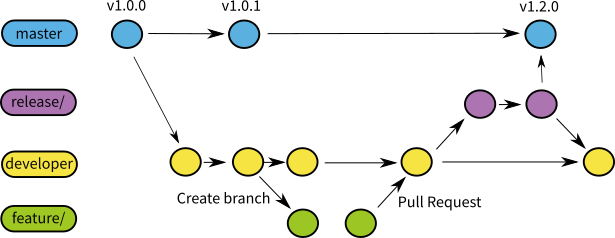
\includegraphics[width=\textwidth]{source/images/pr-flow}
\caption[Visualisierung des \textit{Git-Workflows}.]{Visualisierung des \textit{Git-Workflows}, Quelle: Eigene Darstellung nach \citealt{contribution_workflow}.}
\label{fig:pr-flow}
\end{figure}


\section{\acf{ci}}

Der Begriff \acl{ci}, auch \ac{ci} genannt, entstammt der Software Entwicklung und beschreibt dabei einen Prozess der permanenten Integration. Wie \citet{jenkins-guide} beschreibt, war es in den frühen Anfängen der Softwareentwicklung üblich, dass alle Änderungen der beteiligten Team Mitglieder zu einem Zeitpunkt, der sogenannten Integrationsphase, in der Codebasis vereint wurden und daraus ein \textit{Release} erzeugt wurde. 
Diese Phase ging in der Regel mit harter Arbeit und monatelangem Lösen von Konflikten einher, da diese nur schwer vorherzusehen sind. Noch schwieriger ist es dann, diese zu lösen, da der Code unter Umständen mehrere Monate alt ist. 

Der Prozess der \ac{ci} wurde entwickelt, um diese Probleme zu adressieren. \citet{fowler_2006} merkt an, dass eine \ac{ci} zwar keine \textit{Bugs} beseitigt, es aber deutlich einfacher macht, diese frühzeitig zu finden und zu eliminieren. 
Das Risiko und die Gefahr von unvorhersehbaren Kosten, verspäteten Software-\textit{Releases} und in Folge unglücklicher Kunden wird minimiert \citep{jenkins-guide}.

\autoref{fig:ci-flow} visualisiert einen repräsentativen \ac{ci} unterstützten technischen Prozess.

\begin{figure}[ht!]
\centering
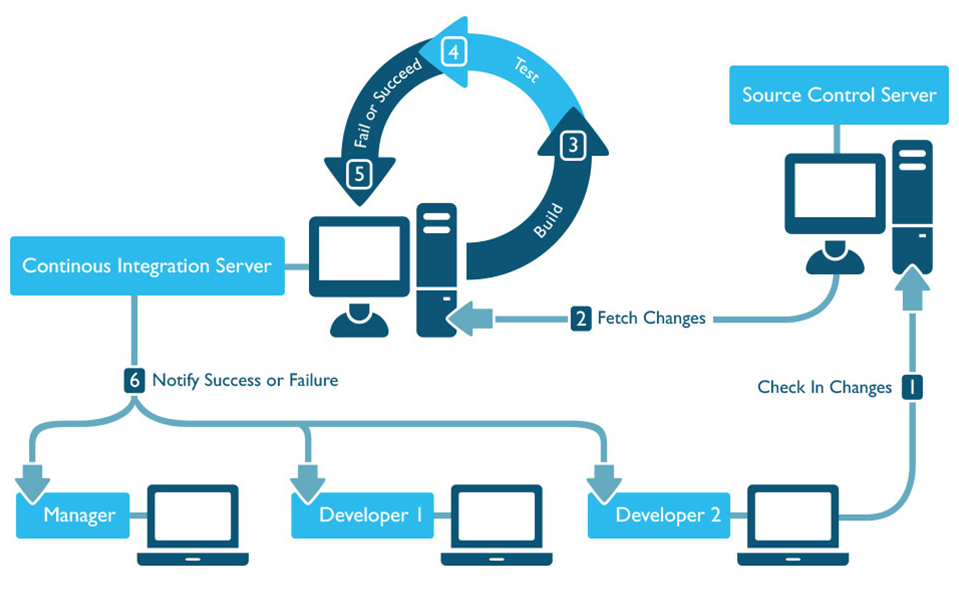
\includegraphics[width=\textwidth]{source/images/ci-flow}
\caption[Technische Umsetzung von \ac{ci}.]{Technische Umsetzung von \ac{ci}, Quelle: \citealt{continuous-improvement}.}
\label{fig:ci-flow}
\end{figure}

Im Wesentlichen beobachtet der \ac{ci}-Server ein \ac{scm} System (2) und führt eine definierte \textit{Build Pipeline} bei jeder Änderung der dazugehörige Codebasis aus (3). So ist es denkbar, dass eine \textit{Build Pipeline} die Codebasis kompiliert, automatisierte Tests ausführt und der Code einer statischen Code Analyse unterzieht (4). Dieser Prozess kann beliebig erweitert und an die Bedürfnisse der einzelnen Teams und deren Projekte angepasst werden. Sollte irgendetwas nicht wie erwartet funktionieren, ein Test fehlschlagen oder gar das Kompilieren der Codebasis misslingen (5), so wird das Team unverzüglich von dem System darüber informiert (6) \citep{jenkins-guide}. 
All das setzt voraus, dass jeder im Team seine \textit{Features} häufig, normalerweise täglich, in das \ac{scm} System integriert (1) \citep{fowler_2006}.

Nach \citet{fowler_2006} ist somit der ganze Sinn einer \ac{ci} schnelles Feedback zu erhalten, um auftretende \textit{Bugs} dadurch frühzeitig zu finden und zu eliminieren, statt diese über lange Zeit in einem \textit{Release} zu kumulieren. Durch die permanente Integration der einzelnen Codebestandteile (\textit{Features}, \textit{Bugfixes}, etc.) wird die Qualität der Software verbessert und Risiken minimiert.

Der \textit{Jenkins} ist ein in \textit{Java} geschriebener \textit{Open Source} \ac{ci}-Server. Die Entwicklung begann im Jahr 2004 durch Kohsuke Kawaguchi, damals unter dem Namen \textit{Hudson} und zählt heute zu den populärsten \ac{ci}-Servern. Dieser wird als Webapplikation bereitgestellt und bietet durch eine große, aktive Community und mehreren hunderten von \textit{Plugins} flexible und diverse Einsatzmöglichkeiten in der permanenten Integration von Softwarekomponenten \citep{jenkins-guide}. \textit{Plugins} bezeichnen Zusatzmodule, die die Basisfunktionalität der eigentlichen Software erweitern. Das \textit{Git Plugin} ermöglicht z.\,B. die Integration eines \textit{Source Code Repositorys} in den \textit{Jenkins}, sodass dieses als Projekt hinzugefügt werden kann und durch den \textit{Jenkins} beobachtet und bei Änderungen analysiert werden kann \citep{git-plugin}.  

\section{Delta-Softwaremetriken}

Nach \citet{augsten_2019} bilden Softwaremetriken bestimmte Eigenschaften von Software als Zahlenwerte ab. Dadurch werden diese vergleichbar und dienen als Maßstab für die Qualität von Software. Beispielsweise bestimmt die \textit{Code Coverage} den prozentualen Anteil des durch automatisierte Tests abgedeckten Quellcodes. Ein Delta bezeichnet im Allgemeinen eine Differenz. 

Eine Delta-Softwaremetrik meint nun die Maßzahl einer bestimmen Softwaremetrik bezogen auf eine Referenz, für die es zwei verschiedene Betrachtungsweisen gibt - die absolute und die relative Referenz.
Bei der absoluten Betrachtung wird als Referenz die gesamte Codebasis des Ziel-\textit{Branches} betrachtet. Das Delta der Metrik gibt also Aufschluss darüber, wie sich die Metrik bezogen auf das Gesamtprojekt durch einen \textit{Pull Request} verändert. 

Ein Beispiel: Auf dem \textit{developer}-\textit{Branch} eines \textit{Repositorys} beträgt die \textit{Code Coverage} 80 \%. Ein Teammitglied entwickelt ein neues \textit{Feature} basierend auf dem \textit{developer}-\textit{Branch} und stellt einen \textit{Pull Request}, damit seine Änderungen in den \textit{developer}-\textit{Branch} integriert werden. Die \textit{Code Coverage} auf dem \textit{feature}-\textit{Branch} beträgt 85 \%. Durch einen erfolgreichen \textit{Merge} wird die \textit{Code Coverage} demnach um 5 \% gesteigert. 

Die relative Betrachtung einer Delta-Metrik bezieht sich dagegen auf den \textit{Pull Request} selbst und gibt an, welche Zeilen des im \textit{Pull Requests} veränderten, gelöschten oder hinzugefügten Quellcodes in der Metrik berücksichtigt sind. 

Ein Beispiel: In einem \textit{Pull Request} wurde der Codebasis eine neue Klasse mit 100 Zeilen hinzugefügt. Für diese Klasse existieren Tests, die den Code automatisiert testen. Diese Tests decken 67 der 100 Zeilen ab. Das bedeutet, dass die Zeilen, die sich in diesem \textit{Pull Request} geändert haben, zu 67 \% durch Tests abgedeckt sind. In der relativen Delta-Betrachtung, besitzt dieser \textit{Pull Request} demnach eine \textit{Code Coverage} von 67 \%. Diese Delta-Betrachtung reduziert die Kennzahl der jeweiligen Softwaremetrik also auf die im \textit{Pull Request} veränderten Codezeilen, anstatt das Gesamtprojekt zu beurteilen. 

Häufig sind es diese Delta-Betrachtungen, die bei einem \textit{Pull Request} relevant sind und für die \textit{Reviewer} von Interesse sind, um die Qualität eines \textit{Pull Requests} und der darin enthaltenen Weiterentwicklung beurteilen zu können. 



\chapter{Methodik und Umsetzung des Plugins}
\label{chap:umsetzung}

\section{Konzeption}

Zu Beginn der Arbeit existierten nur wenige Anforderungen für das in \autoref{chap:einleitung} definierte Ziel, welche der Ausschreibung des Themas dieser Arbeit entstammen und in einem \textit{Abstract} \citep{ausschreibung} verfasst wurden. Nach gemeinsamer Diskussion und Einarbeitung ergaben sich dadurch die im Folgenden beschriebenen Anforderungen.

\begin{table}[H]
\begin{tabularx}{\textwidth} { 
  | X | X | }
 \hline
 Anforderung & \textit{Dashboard} \\
 \hline
Beschreibung  & Das zu entwickelnde \textit{Plugin} soll ein \textit{Dashboard} zur Verfügung stellen, über das die wichtigsten Eigenschaften eines \textit{Pull Requests} visualisiert werden. \\
\hline
\end{tabularx}
\caption{1. Anforderung: \textit{Dashboard}}
\end{table}

\begin{table}[H]
\begin{tabularx}{\textwidth} { 
  | X | X | }
 \hline
 Anforderung & \textit{Portlets} für das \textit{Dashboard} \\
 \hline
Beschreibung  & Die in dem \textit{Dashboard} angezeigten Eigenschaften eines \textit{Pull Requests} sollen durch andere \textit{Plugins} bereitgestellt werden. \\
\hline
\end{tabularx}
\caption{2. Anforderung: \textit{Portlets}}
\label{tab:portlets}
\end{table}

\begin{table}[H]
\begin{tabularx}{\textwidth} { 
  | X | X | }
 \hline
 Anforderung & Konfiguration \\
 \hline
Beschreibung  & Das \textit{Dashboard} soll konfigurierbar sein, d.\,h. der Nutzer kann bestimmen, wie das \textit{Dashboard} aufgebaut ist und welche \textit{Portlets} in welcher Form angezeigt werden. \\
\hline
\end{tabularx}
\caption{3. Anforderung: Konfiguration}
\end{table}

\begin{table}[H]
\begin{tabularx}{\textwidth} { 
  | X | X | }
 \hline
 Anforderung & \ac{api} für andere \textit{Plugins} \\
 \hline
Beschreibung  & Damit andere \textit{Plugins} solche \textit{Portlets} aus \autoref{tab:portlets} bereitstellen können, muss eine \ac{api} konzeptioniert und entwickelt werden. \\
\hline
\end{tabularx}
\caption{4. Anforderung: \ac{api}}
\end{table}

\begin{table}[H]
\begin{tabularx}{\textwidth} { 
  | X | X | }
 \hline
 Anforderung & Distribution \\
 \hline
Beschreibung  & Das zu entwickelnde \textit{Plugin} soll unter der \textit{MIT}-Lizenz als \textit{Jenkins} \textit{Plugin} veröffentlicht werden, sodass dieses über das \textit{Jenkins Update Center} zu finden ist \citep{jenkinsci_plugin_center}. \\ \hline
\end{tabularx}
\caption{5. Anforderung: Distribution}
\end{table}

Die Art und Weise der Umsetzung der einzelnen Anforderungen entschied sich größtenteils erst während der Einarbeitung bzw. der Arbeit selbst, beispielsweise durch das Feedback anderer Entwickler. Da ein neues \textit{Plugin} erschaffen werden sollte, bestanden auch keine Abhängigkeiten zu anderen \textit{Plugins}. Optional wurde als Ziel festgehalten, die ersten \textit{Portlets} in anderen \textit{Plugins} zu implementieren, sodass das \textit{Plugin} im besten Fall im Rahmen dieser Arbeit bereits durch andere Nutzer verwendet werden kann. Zunächst soll in \autoref{chap:realisierung} die technische Realisierung dokumentiert werden, bevor in \autoref{chap:ergebnisse} die Ergebnisse präsentiert werden.

\section{Realisierung}
\label{chap:realisierung}
Im Rahmen der vorliegenden Arbeit wurde ein \textit{Jenkins Plugin} entwickelt. Es wird dessen Entwicklung und die verschiedenen Komponenten erläutert, die zur Umsetzung der in \autoref{chap:umsetzung} definierten Anforderungen maßgebend sind. Zur Veranschaulichung des Zusammenspiels der einzelnen Klassen soll \autoref{fig:uml} dienen. Es zeigt ein vereinfachtes UML-Klassendiagramm der für die zu implementierenden \textit{Plugins} bedeutsamen Klassen. Im Folgenden werden diese erläutert und ihre Funktion beschrieben werden. Aus Gründen der Übersichtlichkeit wird die Code-Dokumentation in den ausgewiesenen Code-Beispielen entfernt. Die jeweilige Originalquelle wird referenziert.

\begin{figure}[H]
\centering
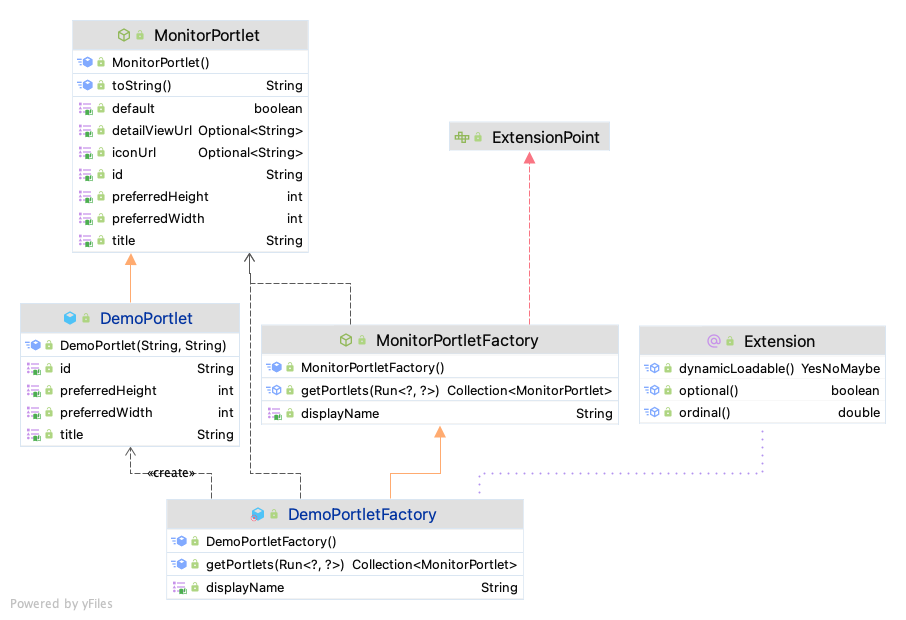
\includegraphics[width=\textwidth]{source/images/uml-with-methods}
\caption[Vereinfachtes UML-Klassendiagramm der für die zu implementierenden \textit{Plugins} relevanten Klassen.]{Vereinfachtes UML-Klassendiagramm der für die zu implementierenden \textit{Plugins} relevanten Klassen, Quelle: Eigene Darstellung.}
\label{fig:uml}
\end{figure}

\subsection{Abstrakte Klassen}
\label{chap:abstractClass}
Die in dem \textit{Plugin} vorhandenen abstrakten Klassen fungieren als Schnittstelle für \textit{Plugins}, die ein \textit{Portlet} bereitstellen möchten. Die beiden abstrakten Klassen \textit{MonitorPortletFactory} und \textit{MonitorPortlet} werden dabei stets zusammen verwendet und stehen in einer \textit{1}:\textit{n}-Beziehung. Jedes \textit{Plugin} besitzt eine \textit{MonitorPortletFactory}, die die \textit{MonitorPortlets} erzeugt und ausliefert. Diese \textit{<<create>>} Beziehung ist in \autoref{fig:uml} veranschaulicht. 
Dadurch wird sichergestellt, dass ein \textit{Plugin} gegebenenfalls mehrere Instanzen der Klasse \textit{MonitorPortlet} bereitstellen kann. Dieser Aspekt ist für die Entwicklung des \textit{Portlets} für das \textit{Warnings Next Generation Plugin} von Bedeutung, welches in \autoref{chap:warnings-ng} vorgestellt wird. Damit das implementierende \textit{Plugin} die beiden Klassen verwenden kann, bedarf es einer Referenz des \textit{Pull Request Monitoring Plugins} in der \textit{pom.xml}, dem \textit{Project Object Model}. Darin werden alle wichtigen Aspekte des Projektes, wie Projektinformationen oder  Projektbeziehungen, also Abhängigkeiten zu anderen Projekten beschrieben. Diese zentrale Steuerungsdatei wird verwendet, um mithilfe des auf \textit{Java} basierenden Build-Managment-Tools \textit{Maven} das Projekt zu verwalten und zu steuern \citep{horn_maven}. Alle \textit{Jenkins} \textit{Plugins} sind in \textit{Java} geschrieben und nutzen dieses Build-Managment-Tool \citep{jenkinsci_plugin}.

\lstinputlisting[escapeinside={(*@}{@*)},caption=Auszug der Datei \textit{plugin/pom.xml} aus dem \textit{Warnings Next Generation Plugin} \citep{warnings-ng-plugin}.,label=listing:pom]{source/listings/pom.xml}

\autoref{listing:pom} demonstriert die Referenzierung anhand des \textit{Warnings Next Generation Plugins}. Zeile \autoref{listing:pom22} deklariert die Abhängigkeit als optional. Dadurch wird diese Abhängigkeit nur dann verwendet, wenn die zugehörige Funktionalität tatsächlich benutzt wird. Wird diese Funktionalität nicht benutzt, so wird auch die Abhängigkeit nicht verwendet.

\subsubsection{\textit{MonitorPortlet}}
Die \textit{MonitorPortlet} Klasse definiert die für ein \textit{Portlet} zu implementierenden Methoden. Ein \textit{Plugin}, welches ein oder mehrere \textit{Portlets} bereitstellen möchte, muss von dieser abstrakten Klasse erben und die Methoden implementieren und gegebenenfalls überschreiben, falls die vordefinierte Implementierung nicht dem jeweiligen Zweck entspricht. \autoref{listing:MonitorPortlet} zeigt die abstrakte Klasse mit ihren Methoden. Ein Titel (vgl. Zeile \autoref{listing:MonitorPortlet3}), eine eindeutige ID (vgl. Zeile \autoref{listing:MonitorPortlet5}), die Breite (vgl. Zeile \autoref{listing:MonitorPortlet11}) und die Höhe (vgl. Zeile \autoref{listing:MonitorPortlet13}) sind in jedem Fall zu implementieren. Zu den optionalen Methoden zählen die Definition eines \textit{Icons} (vgl. Zeile \autoref{listing:MonitorPortlet15}) oder einer Unterseite in Form eines \acp{url} (vgl. Zeile \autoref{listing:MonitorPortlet19}), die geöffnet wird, wenn der Nutzer auf den Titel des im \textit{Dashboard} hinzugefügten \textit{Portlets} klickt. Seit Version 1.7.0 kann ein \textit{Portlet} entscheiden, ob dieses standardmäßig (vgl. Zeile \autoref{listing:MonitorPortlet7}) in jedem \textit{Dashboard} angezeigt werden soll \citep{pull-request-monitoring-plugin}. Näheres dazu wird in \autoref{chap:default} diskutiert.

\lstinputlisting[escapeinside={(*@}{@*)}, language=Java,caption=Auszug der Klasse\\ \textit{io.jenkins.plugins.monitoring.MonitorPortlet.java}\\ \citep{pull-request-monitoring-plugin}.,label=listing:MonitorPortlet]{source/listings/MonitorPortlet.java}

Eine minimalistische Implementierung der \textit{MonitorPortlet} Klasse wird im \textit{Pull Request Monitoring Plugin} mit ausgeliefert und stellt dem Anwender ein erstes beispielhaftes \textit{Portlet} für das \textit{Dashboard} zur Verfügung, welches \autoref{listing:DemoPortlet} zeigt.

\lstinputlisting[escapeinside={(*@}{@*)}, language=Java,caption=Auszug der Klasse \textit{io.jenkins.plugins.monitoring.DemoPortlet.java} \citep{pull-request-monitoring-plugin}.,label=listing:DemoPortlet]{source/listings/DemoPortlet.java}

\textit{Jenkins} realisiert seine \ac{ui} mittels \textit{Jelly}, einer \textit{Java}- und \textit{XML}-basierten Skripting- und Verarbeitungsengine zur Umwandlung von \textit{XML} in ausführbaren Code \citep{strachan_2017}. Die zugehörige \ac{ui}-Komponente eines \textit{MonitorPortlets} wird als \textit{Jelly}-Datei ausgeliefert und trägt den Namen \textit{monitor.jelly}. \textit{Jelly}-Dateien sind direkt an Klassen gebunden. Das bedeutet, dass sie Methoden dieser Klassen aufrufen können. Um die Datei zu referenzieren, an die sie gebunden sind, verwenden \textit{Jelly}-Dateien das Schlüsselwort \texttt{it}. Dabei bedarf es einer bestimmten Verzeichnisstruktur der \textit{Java} Klassen und der \textit{Jelly}-Dateien \citep{jenkins_jelly}. Die \textit{DemoPortlet} Klasse liegt unter \textit{./src/main/java/io/jenkins/plugins/monitoring/DemoPortlet}. Die \textit{Jelly}-Datei, also die \ac{ui}-Komponente zu dieser Klasse liegt dann unter \textit{./src/main/resources/io/jenkins/plugins/monitoring/DemoPortlet/monitor.jelly}. \autoref{listing:DemoPortletMonitor} zeigt die \ac{ui}-Komponente der Klasse \textit{DemoPortlet}.

\lstinputlisting[escapeinside={(*@}{@*)}, language=Java,caption=\textit{io/jenkins/plugins/monitoring/DemoPortlet/monitor.jelly}\\ der Klasse \textit{io.jenkins.plugins.monitoring.DemoPortlet.java} \citep{pull-request-monitoring-plugin}.,label=listing:DemoPortletMonitor]{source/listings/monitor.jelly}

\texttt{it} ist somit die Referenz auf die konkrete Implementierung \textit{DemoPortlet} der abstrakten Klasse \textit{MonitorPortlet}. Zeile \autoref{listing:DemoPortletMonitor5} kann dadurch auf der zugehörigen \textit{Java}-Klasse die Methode aus \autoref{listing:DemoPortlet} Zeile \autoref{listing:DemoPortlet12} ausführen und erhält als Ergebnis den Titel des \textit{Portlets}.

\subsubsection{\textit{MonitorPortletFactory}}

Die Klasse \textit{MonitorPortletFactory} erzeugt die Instanzen der Klasse \textit{MonitorPortlet}. Die abgewandelte Form des \textit{Factory Patterns}, wie es erstmals \citet{gamma_helm_johnson_1998} beschrieben, ermöglicht es den Anwendern, mehrere Instanzen derselben Klasse zu erzeugen, sodass mehrere baugleiche \textit{Portlets} erstellt werden können. Ein \textit{Plugin}, welches ein oder mehrere \textit{Portlets} bereitstellen möchte, muss von dieser abstrakten Klasse erben und die abstrakten Methoden implementieren. \autoref{listing:MonitorPortletFactory} zeigt die Klasse mit ihren abstrakten Methoden.

\lstinputlisting[escapeinside={(*@}{@*)}, language=Java,caption=Auszug der Klasse\\ \textit{io.jenkins.plugins.monitoring.MonitorPortletFactory.java} \citep{pull-request-monitoring-plugin}.,label=listing:MonitorPortletFactory]{source/listings/MonitorPortletFactory.java}

Der Name (vgl. Zeile \autoref{listing:MonitorPortletFactory5}) der \textit{MonitorPortletFactory} dient lediglich der Anzeige im \textit{Dashboard}, unter der alle verfügbaren \textit{Portlets} gelistet sind. Siehe dazu \autoref{fig:add1}.
Eine \textit{MonitorPortletFactory} liefert eine Menge an \textit{MonitorPortlets} aus (vgl. Zeile \autoref{listing:MonitorPortletFactory3}). Diese Methode wiederum wird später verwendet, um die verfügbaren \textit{Portlets} abzurufen. Damit der Inhalt der zu erzeugenden \textit{Portlets} an den jeweiligen \textit{Run} angepasst werden kann, wird der jeweils aktuelle \textit{Run} der Schnittstellenmethode hinzugefügt. 

\autoref{listing:DemoPortletFactory} zeigt die Implementierung der \textit{DemoPortletFactory} der in dem \textit{Pull Request Monitoring Plugin} mit ausgelieferten Demo-\textit{Portlets}. Da diese \textit{Factory} lediglich zwei statische \textit{Portlets} ausliefert und nur der Demonstration dient, wird der übergebene \textit{Run} ignoriert. In einer realen Implementierung, wie der aus \autoref{chap:warnings-ng} und \autoref{chap:code-coverage-api}, werden über diesen \textit{Run} Informationen abgegriffen, um den Inhalt der \textit{Portlets} entsprechend anzupassen.

\lstinputlisting[escapeinside={(*@}{@*)}, language=Java,caption=Auszug der statischen Klasse\\ \textit{io.jenkins.plugins.monitoring.DemoPortletFactory.java}\\ der Klasse \textit{io.jenkins.plugins.monitoring.DemoPortlet.java} \citep{pull-request-monitoring-plugin}.,label=listing:DemoPortletFactory]{source/listings/DemoPortletFactory.java}

\subsection{Das Konzept \textit{ExtensionPoint} des \textit{Jenkins}}

Ein wesentliches Konzept des \textit{Jenkins} besteht darin, die Kernfunktionalität durch \textit{Plugins} erweitern zu können. Dafür stellt der \textit{Jenkins} Erweiterungspunkte in Form von Schnittstellen oder abstrakten Klassen zur Verfügung, die die \textit{Plugins} nutzen können, um eine Implementierung beizusteuern. Ein \textit{Plugin} selbst kann dann wiederum eigene \textit{ExtensionPoints} definieren, die von weiteren \textit{Plugins} verwendet werden können, wie in dem vorliegenden Beispiel der Klasse \textit{MonitorPortletFactory}.
Die Markierungsschnittstelle (\textit{Marker Interface)} {ExtensionPoint}, die von der abstrakte Klasse \textit{MonitorPortletFactory} implementiert wird (vgl. \autoref{listing:MonitorPortletFactory}), dient dazu, dem \textit{Jenkins} zur Laufzeit Informationen über die implementierende Klasse der \textit{MonitorPortletFactory} zu liefern. Durch das Scannen aller verfügbaren Klassen innerhalb des \textit{Java Classpaths} werden alle Klassen gefunden, die die abstrakte Klasse und somit den \textit{ExtensionPoint} implementieren. Die entsprechende Implementierung wird registriert und dem \textit{Jenkins} bekannt gemacht. Durch die Annotation der Klasse mit \textit{@Extension} (vgl. \autoref{listing:DemoPortletFactory}, Zeile \autoref{listing:DemoPortletFactory1}) wird eine Instanz der Klasse erzeugt und in der \textit{ExtensionList} des \textit{Jenkins} registriert. Sofern die Abhängigkeit zu dem \textit{Pull Request Monitoring Plugin} in der \textit{pom.xml} aus \autoref{listing:pom} als optional deklariert ist, muss auch die Annotation \textit{Extension} als optional markiert sein. 
\autoref{listing:PortletService} zeigt die Anwendung der \textit{ExtensionList}, um die registrierten Instanzen der \textit{MonitorPortletFactory} Klasse auszulesen. Diese Klasse \textit{PortletService} stellt diverse statische Methoden zur Verfügung, um mit der \textit{ExtensionList} des \textit{Jenkins} zu interagieren und die Implementierungen der abstrakten Klassen aus \autoref{chap:abstractClass} anderer \textit{Plugins} auszulesen. Die Verwendung der Klasse wird in \autoref{chap:MonitoringDefaultAction} näher beschrieben.

\lstinputlisting[escapeinside={(*@}{@*)}, language=Java,caption=Auszug der Klasse\\ \textit{io.jenkins.plugins.monitoring.util.PortletService.java} \citep{pull-request-monitoring-plugin}.,label=listing:PortletService]{source/listings/PortletService.java}

\subsection{Konfiguration}
Die Konfiguration des \textit{Dashboards}, also die in einem \textit{Dashboard} verwendeten \textit{Portlets}, wird pro Projekt gespeichert. Ein Projekt meint dabei in der Regel immer ein \ac{scm}-\textit{Repository}. Für einen Nutzer werden sämtliche Konfigurationen aller \textit{Dashboards} zusammen mit einer eindeutigen ID des zugehörigen Projekts als Liste in einer \textit{UserProperty}, der \textit{MonitorConfigurationProperty}, gespeichert. Diese Klasse stellt einige Methoden zur Verfügung, um die Liste der Konfigurationen abzufragen oder zu bearbeiten. Durch einen statische \textit{Factory}-Methode \citep{gamma_helm_johnson_1998} kann die für den aktuellen Nutzer vorhandene \textit{MonitorConfigurationProperty} erfragt werden.

\lstinputlisting[escapeinside={(*@}{@*)}, language=Java,caption=Auszug der Klasse\\ \textit{io.jenkins.plugins.monitoring.MonitorConfigurationProperty.java} \citep{pull-request-monitoring-plugin}.,label=listing:MonitorConfigurationProperty]{source/listings/MonitorConfigurationProperty.java}

Sollte kein Nutzer eingeloggt sein, so liefert die Methode aus \autoref{listing:MonitorConfigurationProperty} kein Ergebnis. Die \textit{MonitorConfigurationProperty} hält stets eine \textit{default} Konfiguration in der Liste, die geladen wird, wenn der Nutzer das jeweilige \textit{Dashboard} das erste Mal öffnet oder für das Projekt keine anderweitige Konfiguration vorhanden ist. Die \textit{default} Konfiguration enthält dabei immer diejenigen \textit{Portlets}, deren Methode aus \autoref{listing:MonitorPortlet} Zeile \autoref{listing:MonitorPortlet7} \textit{true} zurückliefert. Diese \textit{default} Konfiguration des \textit{Dashboards} kann durch den Nutzer auf zwei unterschiedliche Wege verändert werden: Entweder über das \ac{ui} des \textit{Dashboards} oder die \textit{Pipeline}.

\subsection{\textit{Pipeline}} 
Eine Pipeline ist eine Sammlung von Schritten, die für ein bestimmtes Projekt definiert und ausgeführt werden. Üblicherweise wird eine \textit{Pipeline} in \textit{Jenkins} als \textit{Jenkinsfile} benannt. Die \textit{Pipeline} ist eine typische Charakteristik des \ac{ci} Prozesses, die dafür sorgt, dass die Software oder allgemeiner das Projekt von dem \ac{scm} \textit{Repository} in ein an den Kunden auslieferbares Produkt überführt wird \citep{pipeline, dev-ops-handbuch}. Verschiedene Schritte, sogenannte \textit{Build-Jobs} werden dadurch zu einem \textit{Workflow} zusammengefasst und in einer Datei, dem \textit{Jenkinsfile}, als \textit{Groovy}-Code beschrieben \citep{apache-software-foundation}. Das \textit{Pull Request Monitoring Plugin} stellt einen \textit{Build-Job} zur Verfügung, womit der Nutzer das \textit{Dashboard} vorkonfigurieren kann. \autoref{listing:Jenkinsfile} zeigt lediglich die entsprechende \textit{Stage} des \textit{Jenkinsfiles}, in der die Konfiguration für das \textit{Dashboard} definiert wird. 
\textit{Stages} in \textit{Jenkinsfiles} dienen dazu, den \textit{Code} zu strukturieren und konzeptionell gegenüber anderen \textit{Stages} abzugrenzen. Üblicherweise findet man in einem \textit{Jenkinsfile} eine \textit{Build}-, \textit{Test}- und \textit{Deploy}-\textit{Stage} \citep{pipeline}. 

\lstinputlisting[escapeinside={(*@}{@*)}, caption=\textit{Pull Request Monitoring} \textit{Stage} eines\\ \textit{Jenkinsfiles} \citep{pull-request-monitoring-plugin}.,label=listing:Jenkinsfile]{source/listings/Jenkinsfile}

Bei dieser Konfiguration werden die beiden durch das \textit{Pull Request Monitoring Plugin} ausgelieferten Demo-\textit{Portlets} konfiguriert. Der Nutzer hat die Möglichkeit von der Breite, der Höhe und der Farbe der Implementierung des \textit{Portlets} abzuweichen und diese zu überschreiben. Die Konfiguration wird dabei als \textit{JSON} beschrieben. Durch Zeile \autoref{listing:Jenkinsfile2} wird der \textit{Code} im \textit{Jenkinsfile} mit der entsprechenden \textit{Java}-Klasse, dem \textit{Monitor} verknüpft. Dieser \textit{Step} wird im Kontext des \textit{Workflows} ausgeführt und dadurch zu gegebenem Zeitpunkt die zugehörige \textit{Java}-Klasse aufgerufen. Die \textit{Java}-Klasse fügt eine \textit{MonitoringCustomAction} mit der definierten Konfiguration dem entsprechenden \textit{Run} hinzu, was \autoref{listing:Monitor} zeigt.

\lstinputlisting[escapeinside={(*@}{@*)}, language=Java, caption=Auszug des \textit{Steps} \textit{io.jenkins.plugins.monitoring.Monitor.java} \citep{pull-request-monitoring-plugin}.,label=listing:Monitor]{source/listings/Monitor.java}


\subsection{\textit{Actions}}
\label{chap:actions}
\textit{Actions} sind im Allgemeinen Objekte, die es ermöglichen Informationen zu speichern und \ac{ui}-Elemente dem \textit{Jenkins} hinzuzufügen. Jede \textit{Action} definiert dabei einen Unterbereich innerhalb des aktiven \textit{ModelObjects} des \textit{Jenkins}. Ein \textit{ModelObject} ist eine Schnittstelle, die von \textit{Actions} implementiert wird und definiert, dass die implementierende \textit{Action} eine \ac{url} zur Verfügung stellen muss. Über die definierte \ac{url} kann der Nutzer mit dem \ac{ui} interagieren und den durch die \ac{url} definierten Unterbereich aufrufen. Eine \textit{Action} zu einem \textit{ModelObject} wird immer auch in der Menüleiste des \textit{Jenkins} angezeigt. Die für das \textit{Pull Request Monitoring Plugin} wichtigen \textit{ModelObjects} beschränken sich auf den \textit{Job} und den \textit{Run}. Das \textit{Pull Request Monitoring Plugin} nutzt insgesamt vier solcher \textit{Actions}. 
Das \textit{ModelObject} System lässt sich am besten an den durch die \textit{Actions} definierten \acp{url} veranschaulichen. \autoref{fig:url} zeigt die gesamte \ac{url} einer \textit{MonitoringDefaultAction}, anhand derer die einzelnen \textit{ModelObjects} erkennbar sind.

\begin{figure}[ht!]

$\overbrace{localhost:8080/jenkins/}^{1.}\overbrace{job/}^{2.}\overbrace{PullRequestMonitoringPlugin/}^{3.} \\
\underbrace{view/change-requests/}_{4.}\underbrace{job/}_{5.}\underbrace{PR-2/}_{6.}\underbrace{3/}_{7.}\underbrace{pull-request-monitoring/}_{8.} $

\caption[\ac{url} einer \textit{MonitoringDefaultAction}.]{\ac{url} einer \textit{MonitoringDefaultAction}, Quelle: Eigene Darstellung.}
\label{fig:url}
\end{figure}

\begin{enumerate}
	\item Root \ac{url} des \textit{Jenkins}-Servers.
	\item Typ des \textit{ModelObjects} erster Ebene (\textit{Job}).
	\item Name des \textit{Jobs} erster Ebene. Dieser \textit{Job} ist das \textit{MultiBranchProject}.
	\item Spezifische \acp{url} des \textit{MultiBranchProjects}.
	\item Typ des \textit{ModelObjects} zweiter Ebene (\textit{Job}).
	\item Name des \textit{Jobs} zweiter Ebene. Dieser \textit{Job} repräsentiert beispielsweise einen \textit{Pull Request} und entspricht einem \textit{WorkflowJob}.
	\item Typ des \textit{ModelObjects} dritter Ebene (\textit{Run}). Dem Namen des \textit{Runs} (hier der dritte \textit{Run}) steht anders als den \textit{ModelObjects} erster und zweiter Ebene nicht der Typ voran.
	\item Spezifische \ac{url} der \textit{MonitoringDefaultAction}. Darüber ist das \textit{Dashboard} erreichbar.
 \end{enumerate}
 
Das verknüpfte \ac{scm}-\textit{Repository} wird als \textit{MultiBranchProject} dem \textit{Jenkins} hinzugefügt und bildet den hierarchischen Knotenpunkt (2, 3). Für dieses \textit{ModelObject} vom Typ \textit{Job} definiert das \textit{Pull Request Monitoring Plugin} eine \textit{MonitoringMultibranchProjectAction}. Diese gibt einen ersten Überblick über das Projekt und wird in \autoref{chap:job-result} näher vorgestellt.
Ein \textit{MultiBranchProject} zeichnet sich dadurch aus, dass jeder \textit{Branch} und jeder \textit{Pull Request} als eigenes \textit{ModelObject} (\textit{Job}) angesehen wird und hierarchisch unter dem \textit{ModelObject} des \textit{MultiBranchProjects} geführt wird (3 - 6). Auf dieser Ebene stellt das \textit{Pull Request Monitoring Plugin} die \textit{MonitoringWorkflowJobAction} zur Verfügung. Diese \textit{Action} referenziert lediglich den aktuellsten \textit{Run} des zugehörigen \textit{Jobs} der zweiten Hierachiebene. Ein \textit{Job} dieser Ebene (5), welcher z.\,B. einen bestimmten \textit{Pull Request} aus dem verknüpften \ac{scm}-\textit{Repository} abbildet (6), besitzt in der Regel eine Menge an \textit{ModelObjects} des Typs \textit{Run} (7). Ein \textit{Run} definiert dabei die unterste Ebene des \textit{ModelObjetcs}. Hier wird das eigentliche \textit{Dashboard} für jeden \textit{Run} in Form einer \textit{MonitoringDefaultAction} bereitgestellt (8). 

\subsubsection{\textit{MonitoringCustomAction}}
Eine \textit{MonitoringCustomAction} speichert die nutzerspezifische Konfiguration aus dem \textit{Jenkinsfile}. Diese ist eine unsichtbare \textit{Action} und wird nicht in dem \ac{ui} des \textit{Jenkins} angezeigt. 
Bestehende \textit{Actions}, die einem \textit{Run} hinzugefügt wurden, können nicht mehr verändert werden. Da die \textit{MonitoringDefaultAction} in jedem Fall einem \textit{Run} hinzugefügt wird, sobald dieser geöffnet wird, bedarf es dieser zusätzlichen \textit{Action} im Falle der Konfiguration über eine \textit{Pipeline}. Diese \textit{Action} wird dem \textit{Run} erst hinzugefügt, wenn der entsprechende \textit{Step} der \textit{Pipeline} ausgeführt wurde. 

\subsubsection{\textit{MonitoringDefaultAction}}
\label{chap:MonitoringDefaultAction}
Jedem \textit{Run} innerhalb eines \textit{Multibranch} Projekts wird die \textit{MonitoringDefaultAction} zugeordnet, sofern es sich um einen \textit{Run} im Kontext eines \textit{Pull Requests} handelt. Diese ist über das Menü erreichbar und stellt das eigentliche \textit{Dashboard} bereit. 

Die jeweils gültige Konfiguration zu dem \textit{Dashboard} wird zur Laufzeit ermittelt. \autoref{listing:MonitoringDefaultAction} zeigt die darin involvierten Methoden der \textit{MonitoringDefaultAction}.

\lstinputlisting[escapeinside={(*@}{@*)},language=Java,caption=Auszug der Klasse\\ \textit{io.jenkins.plugins.monitoring.MonitoringDefaultAction.java} \citep{pull-request-monitoring-plugin}.,label=listing:MonitoringDefaultAction]{source/listings/MonitoringDefaultAction.java}

Existiert eine entsprechende Konfiguration für das aktuelle Projekt in der \textit{MonitoringConfigurationProperty} (vgl. Zeile \autoref{listing:MonitoringDefaultAction16}), so wird diese angewendet. Besteht keine Konfiguration für das Projekt, so liefert die Abfrage der Konfiguration die \textit{default}-Konfiguration. 

Wenn keine \textit{MonitoringConfigurationProperty} für den aktuellen Nutzer vorhanden ist (vgl. Zeile \autoref{listing:MonitoringDefaultAction15}), weil dieser zum Beispiel nicht eingeloggt ist, so wird entweder die \textit{default}-Konfiguration angewendet (vgl. Zeile \autoref{listing:MonitoringDefaultAction27} und \autoref{listing:MonitoringDefaultAction32}) oder falls eine \textit{MonitoringCustomAction} existiert (vgl. Zeile \autoref{listing:MonitoringDefaultAction28}), die darin enthaltene Konfiguration verwendet. Die \ac{ui}-Komponente einer \textit{Action} wird durch die zugehörige \textit{Jelly}-Datei beschrieben.

\lstinputlisting[escapeinside={(*@}{@*)}, linerange={1-6, 20-21, 44-54, 61-62, 68}, caption=Auszug der Datei\\ \textit{io/jenkins/plugins/monitoring/MonitoringDefaultAction/index.jelly} \citep{pull-request-monitoring-plugin}.,label=listing:MonitoringDefaultActionJelly]{source/listings/index.jelly}

Zeile \autoref{listing:MonitoringDefaultActionJelly20} und \autoref{listing:MonitoringDefaultActionJelly21} binden zwei weitere \textit{Plugins} ein, die die externen \textit{JavaScript} Bibliotheken \textit{Muuri} und \textit{Select2} über ein \textit{Jenkins} \textit{Plugin} zur Verfügung stellen \citep{muuri-api-plugin, select2-api-plugin}. \textit{Muuri} liefert ein sortierbares, filterbares und verschiebbares Layout, in das die \textit{Portlets} eingebettet werden \citep{muuri}. \textit{Select2} sorgt dafür, dass die Liste der verfügbaren \textit{Portlets} durchsucht und gefiltert werden kann \citep{select2}. Das Ergebnis wird in \autoref{chap:build-result} vorgestellt.

Zeile \autoref{listing:MonitoringDefaultActionJelly44} dient der Einführung des \textit{Muuri} Layouts und definiert die äußere Form des \textit{Dashboards}. \textit{Muuri} erlaubt es, in dieses Layout einzelne \textit{Items} einzubetten.

In Zeile \autoref{listing:MonitoringDefaultActionJelly46} werden alle verfügbaren \textit{Portlets} durch den \textit{PortletService} aus \autoref{listing:PortletService} ermittelt. Dazu werden alle \textit{MonitorPortletFactory} Instanzen, die in der \textit{ExtensionList} registriert sind, abgerufen und die jeweiligen \textit{MonitorPortlets} erfragt. Für jedes dieser \textit{MonitorPortlet} Objekte (vgl. Zeile \autoref{listing:MonitoringDefaultActionJelly48}) wird eine weitere \textit{Jelly}-Datei inkludiert und die jeweilige \textit{MonitorPortlet} Instanz als Attribut übergeben (vgl. Zeile \autoref{listing:MonitoringDefaultActionJelly50}). \autoref{listing:PortletJelly} zeigt die zu inkludierende \textit{Jelly}-Datei.

\lstinputlisting[escapeinside={(*@}{@*)}, caption=Auszug der Datei \textit{portlet/portlet.jelly} \citep{pull-request-monitoring-plugin}.,label=listing:PortletJelly]{source/listings/portlet.jelly}

Für jedes \textit{MonitorPortlet} wird das eigentliche \textit{Item} erzeugt und dieses dem Layout aus \autoref{listing:MonitoringDefaultActionJelly} Zeile \autoref{listing:MonitoringDefaultActionJelly44} untergeordnet. Die spezifischen Attribute jedes \textit{MonitorPortlets} werden als HTML-Attribute dem \textit{Item} hinzugefügt (vgl. Zeile \autoref{listing:PortletJelly14}) und die \ac{ui}-Komponete des jeweiligen \textit{Portlets} ebenfalls als \textit{Jelly}-Datei inkludiert (vgl. Zeile \autoref{listing:PortletJelly37}). 

Initial werden alle \textit{Portlets} dem Layout als unsichtbares \textit{Item} durch die Zuweisung der \textit{CSS}-Klasse \textit{hidden} aus \autoref{listing:PortletJelly} Zeile \autoref{listing:PortletJelly14} hinzugefügt. Die jeweils gültige Konfiguration wird dann mit den in dem Layout vorhandenen \textit{Items} abgeglichen und die Attribute der \textit{Items}, z.\,B. Höhe, Breite oder Farbe gegebenenfalls angepasst. Anschließend werden die vom Nutzer gewünschten \textit{Portlets} durch das Entfernen der \textit{CSS}-Klasse \textit{hidden} wieder sichtbar gemacht.

Die Verwaltung der \textit{Portlets} geschieht in einer spezifischen \textit{JavaScript}-Datei \textit{pull-request-monitoring.js}. Die \textit{MonitoringDefaultAction} wird ständig über Änderungen informiert und persisitiert diese in der \textit{MonitorConfigurationPrtoperty}. Ähnlich wie mit dem Schlüsselwort \textit{it} einer \textit{Jelly}-Datei, kann auch aus einer \textit{JavaScript}-Datei auf \textit{Java-Klassen} zugegriffen werden und die darin definierten Methoden aufgerufen werden. Dazu wird in \autoref{listing:MonitoringDefaultActionJelly} Zeile \autoref{listing:MonitoringDefaultActionJelly61} die Instanz der \textit{MonitoringDefaultAction} einer Variablen \textit{run} innerhalb eines script-Tags zugewiesen. In Zeile \autoref{listing:MonitoringDefaultActionJelly62} wird dann die spezifische \textit{JavaScript}-Datei eingebunden. Darin wird über die Variable \textit{run} die gültige Konfiguration aus der \textit{MonitoringDefaultAction} abgerufen und die bereits bestehenden \textit{Items} des \textit{Muuri} Layouts entsprechend angepasst. Das Abrufen und Inititialisieren erfolgt in \autoref{listing:js}.


\lstinputlisting[escapeinside={(*@}{@*)}, caption=Auszug der Datei \textit{pull-request-monitoring.js} \citep{pull-request-monitoring-plugin}.,label=listing:js]{source/listings/pull-request-monitoring.js}


\chapter{Ergebnisse}
\label{chap:ergebnisse}

Nachdem in \autoref{chap:umsetzung} bereits die technische Erklärung der einzelnen Bestandteile erfolgte, werden nun die für den Anwender wichtigen Ergebnisse innerhalb des \textit{Jenkins} \ac{ui} dargestellt.

\section{\acl{ui} des Plugins} 

Das \textit{Plugin} bietet, wie in \autoref{chap:actions} eingeführt, zwei \textit{Actions} mit einer \ac{ui}-Komponente. Eine Übersicht über alle \textit{Pull Requests} auf erster \textit{Job}-Ebene und das eigentliche \textit{Dashboard} auf der \textit{Run}-Ebene.

\subsection{\textit{Job}-Ansicht}
\label{chap:job-result}

Für jeden \textit{Pull Request} werden der Name des \textit{Pull Requests}, der Name des Mitwirkenden und sowohl der Quell- als auch der Ziel-\textit{Branch} aufgelistet, wie \autoref{fig:overview} zeigt. 

\begin{figure}[h!]
\centering
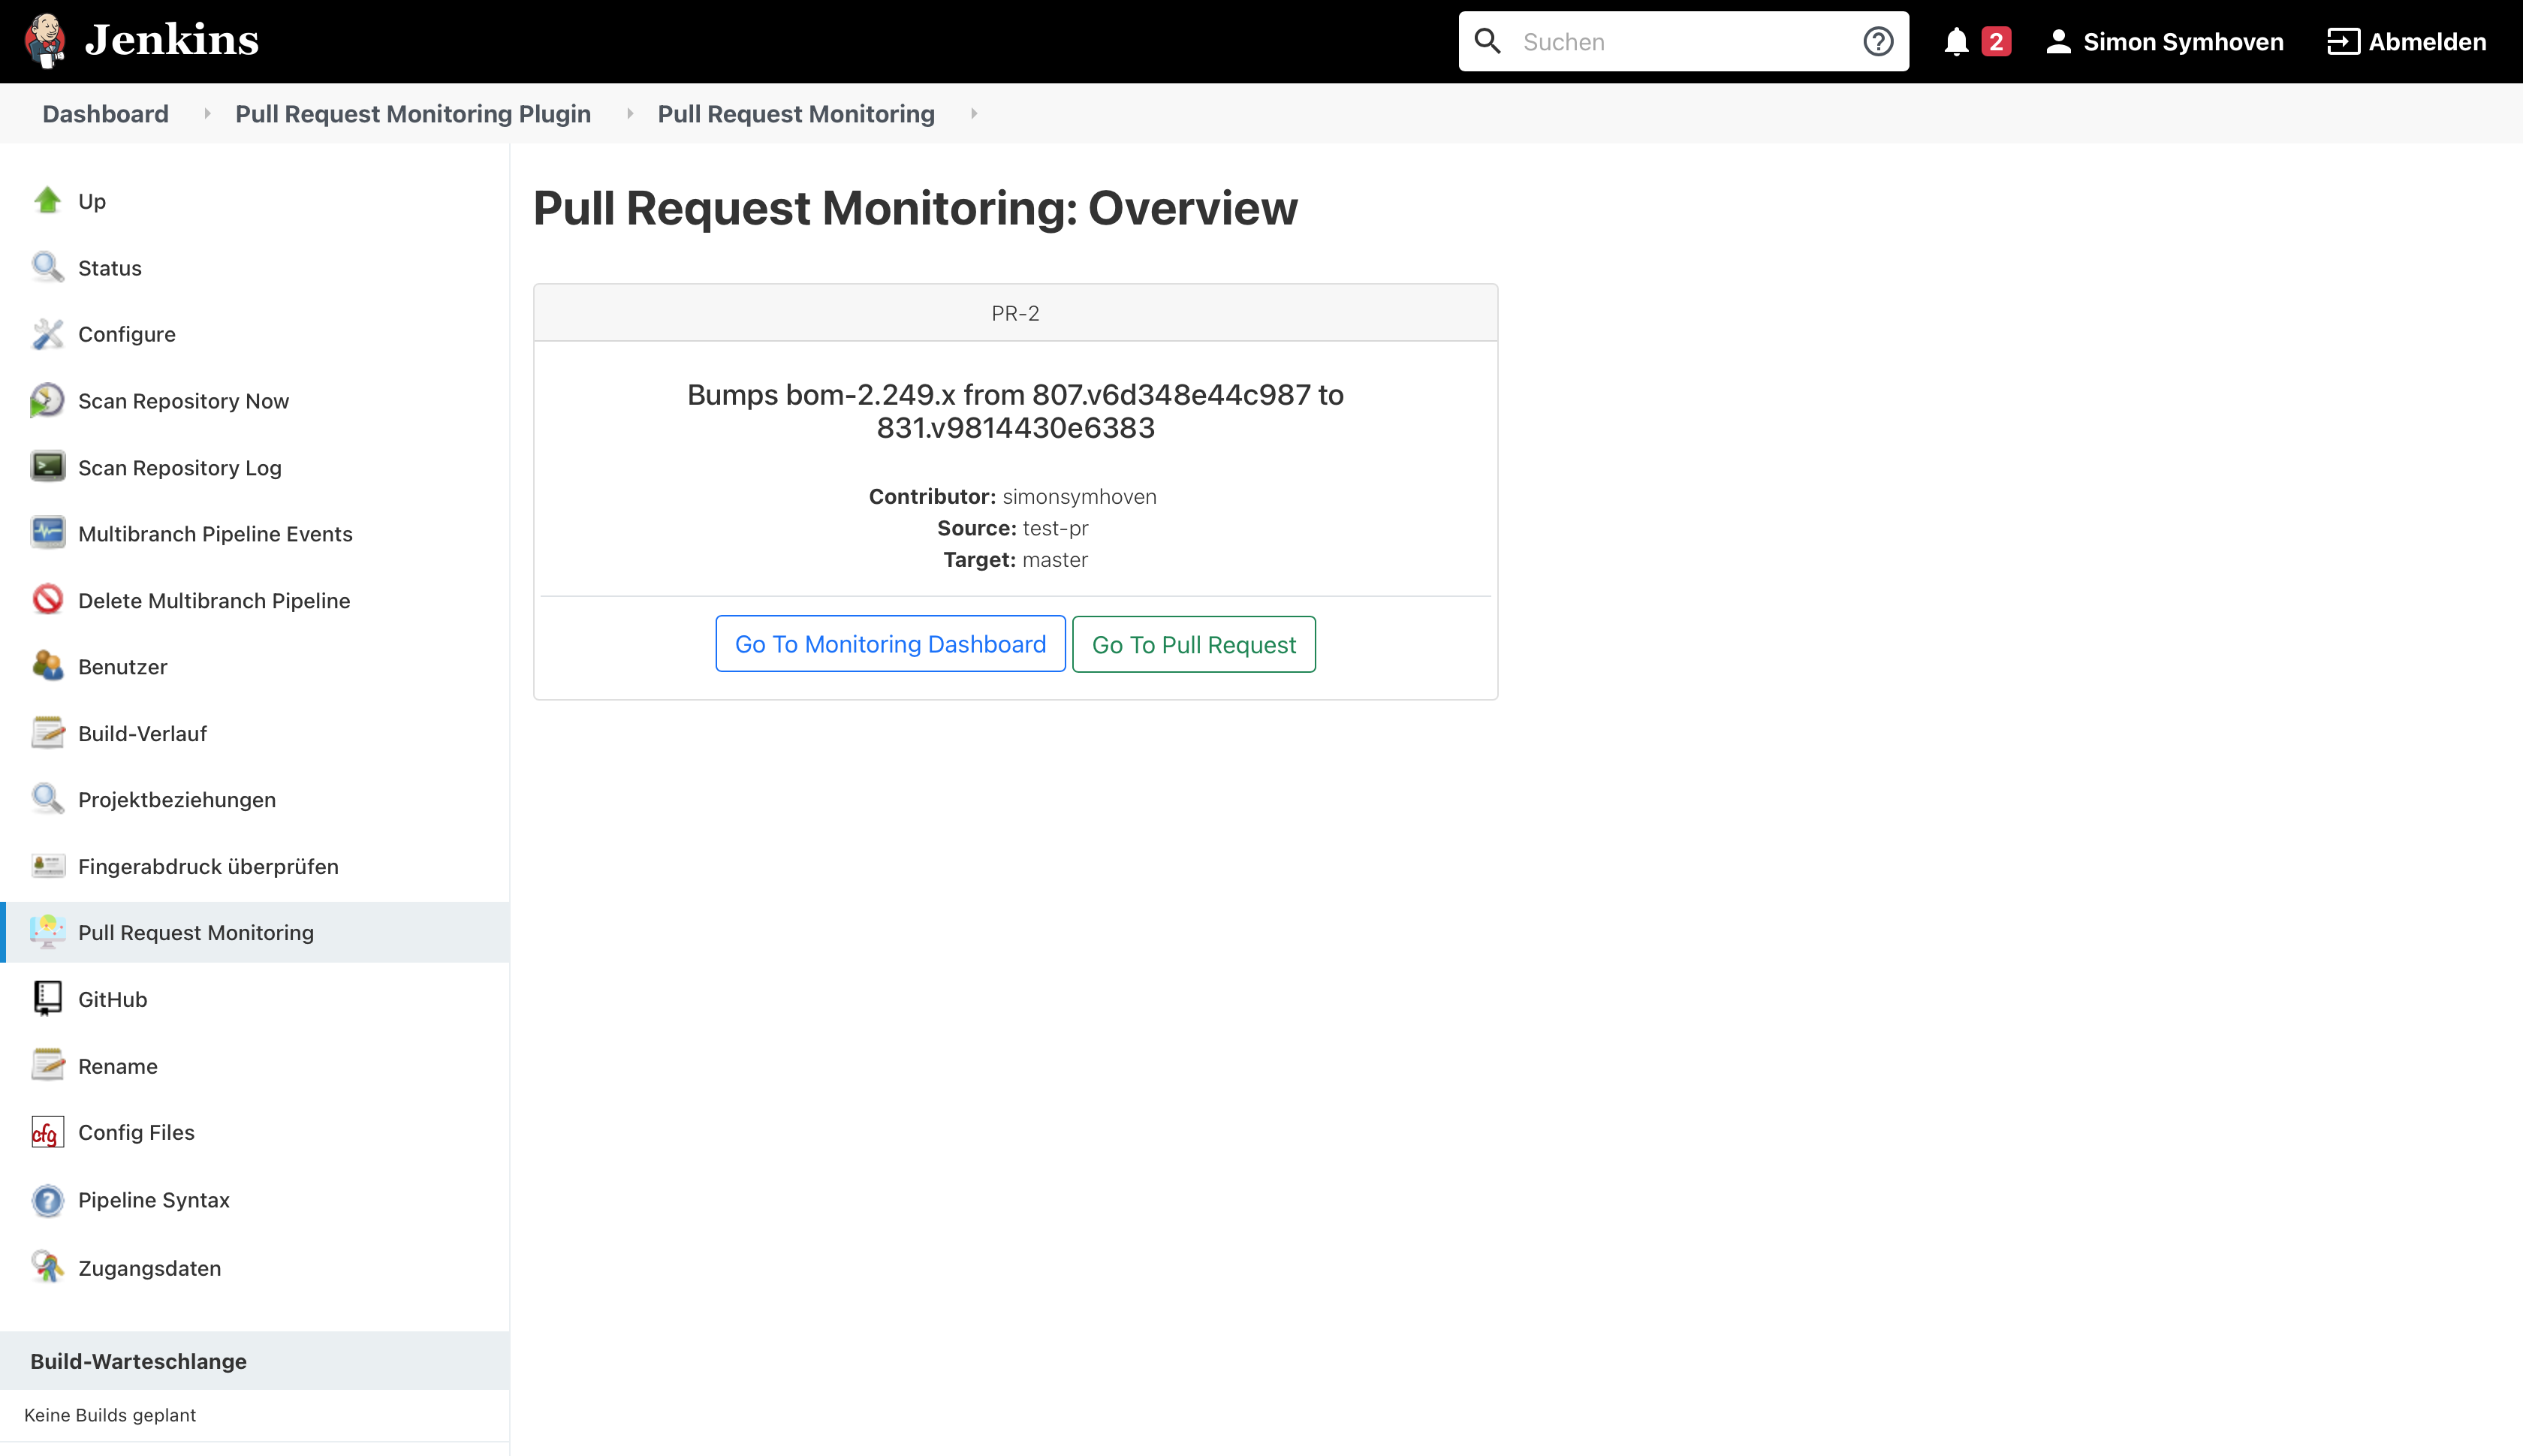
\includegraphics[width=\textwidth]{source/images/overview}
\caption[\textit{MonitoringMultibranchProjectAction} auf erster \textit{Job}-Ebene: Übersicht aller \textit{Pull Requests}.]{\textit{MonitoringMultibranchProjectAction} auf erster \textit{Job}-Ebene: Übersicht aller \textit{Pull Requests}, Quelle: Eigene Aufnahme.}
\label{fig:overview}
\end{figure}

Von hier aus kann entweder zu der \ac{ui}-Komponente des letzten zugehörigen \textit{Runs}, also der \textit{Run}-Ansicht aus \autoref{chap:build-result} mit dem \textit{Dashboard} navigiert werden oder der \textit{Pull Request} im \ac{scm}-System, z.\,B. \textit{GitHub} geöffnet werden.


\subsection{\textit{Run}-Ansicht}
\label{chap:build-result}

Das \textit{Dashboard} besteht aus verschiedenen Einheiten. Einem Titel, den Metadaten eines \textit{Pull Requests}, dem \textit{Muuri} Layout mit den \textit{Portlets} und zwei Schaltflächen, um neue \textit{Portlets} hinzuzufügen und die Einstellungen zu öffnen. 

\begin{figure}[h!]
\centering
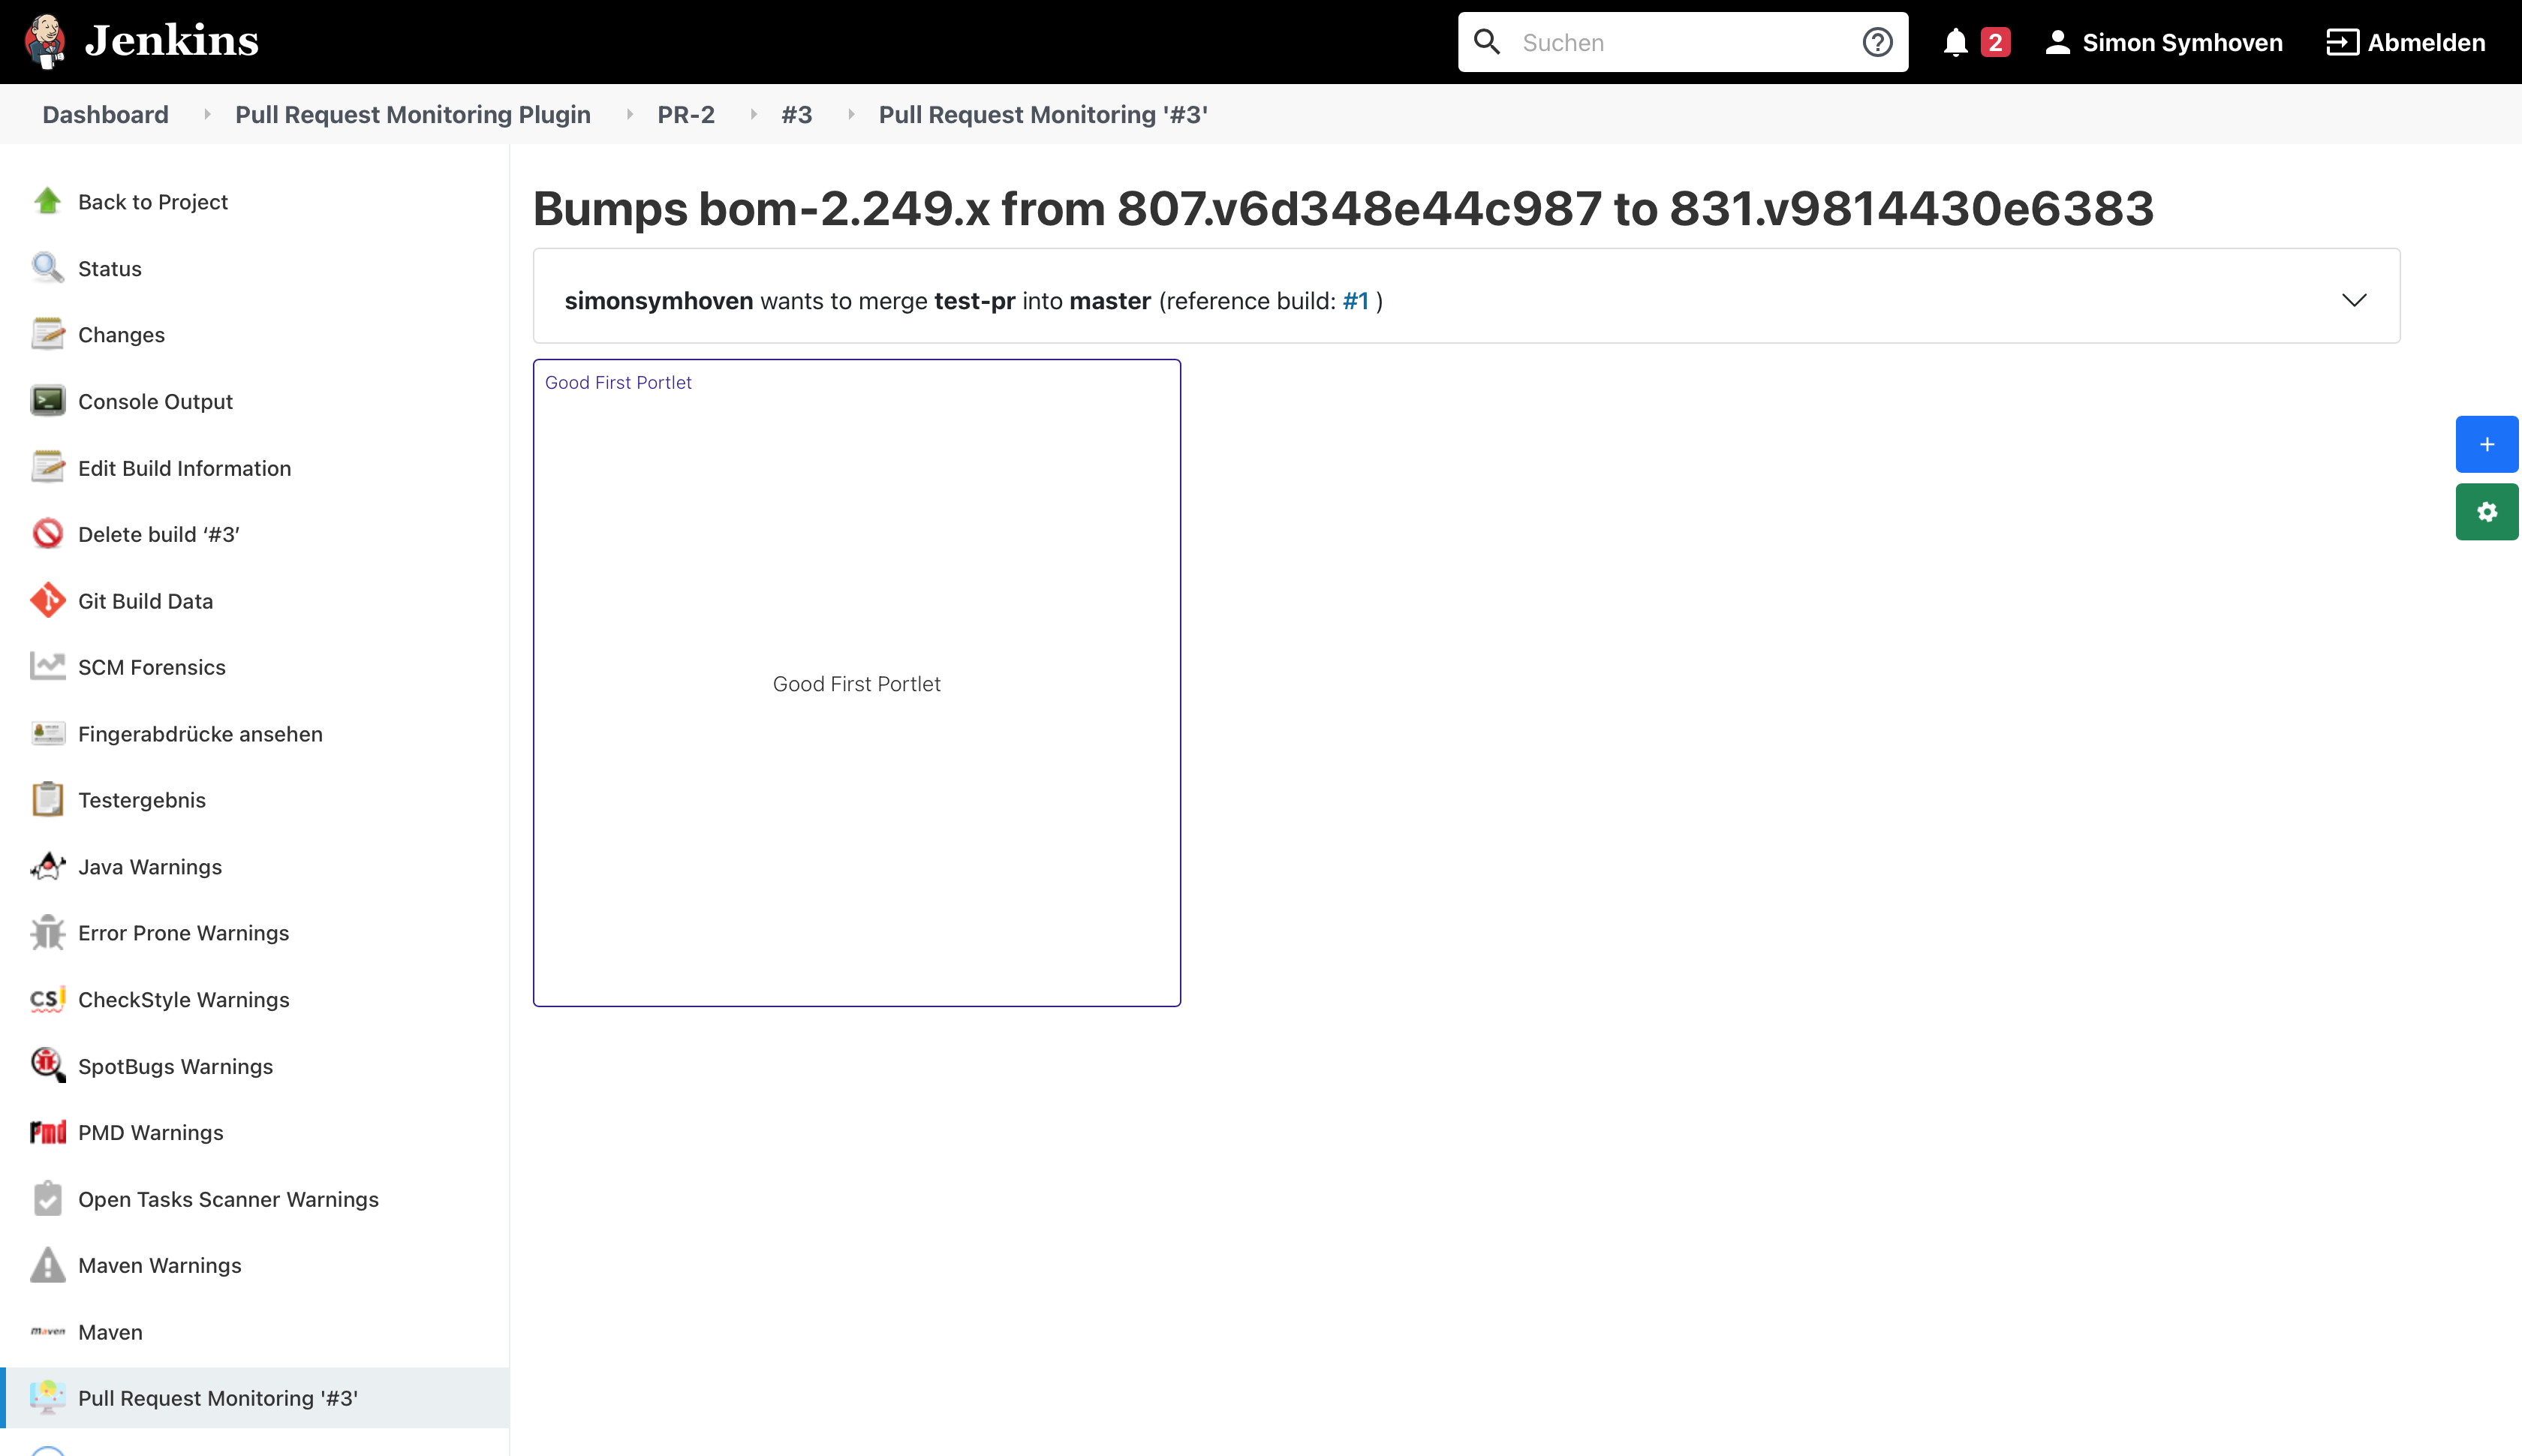
\includegraphics[width=\textwidth]{source/images/build}
\caption[\textit{MonitoringDefaultAction} auf \textit{Run}-Ebene: Das \textit{Dashboard}.]{\textit{MonitoringDefaultAction} auf \textit{Build}-Ebene: Das \textit{Dashboard}, Quelle: Eigene Aufnahme.}
\label{fig:build}
\end{figure}

Die \textit{Portlets} innerhalb des \textit{Muuri} Layouts aus \autoref{fig:build} können per \textit{Drag \& Drop} beliebig verschoben werden oder mit einem Klick auf die rechte obere Ecke des jeweiligen \textit{Portlets} gelöscht werden.

\subsubsection{Metadaten eines \textit{Pull-Requests}}

Analog zu der Übersicht der \textit{Pull Requests} aus \autoref{chap:job-result} werden auf \textit{Run}-Ebene alle Metadaten des \textit{Pull Requests} angezeigt. Außerdem wird der Referenz-\textit{Run} des zugehörigen Ziel-\textit{Branches} angegeben. Zusätzlich wird, falls vorhanden, die Beschreibung aus dem \ac{scm}-System ausgegeben, wie \autoref{fig:metadata} zeigt:

\begin{figure}[h!]
\centering
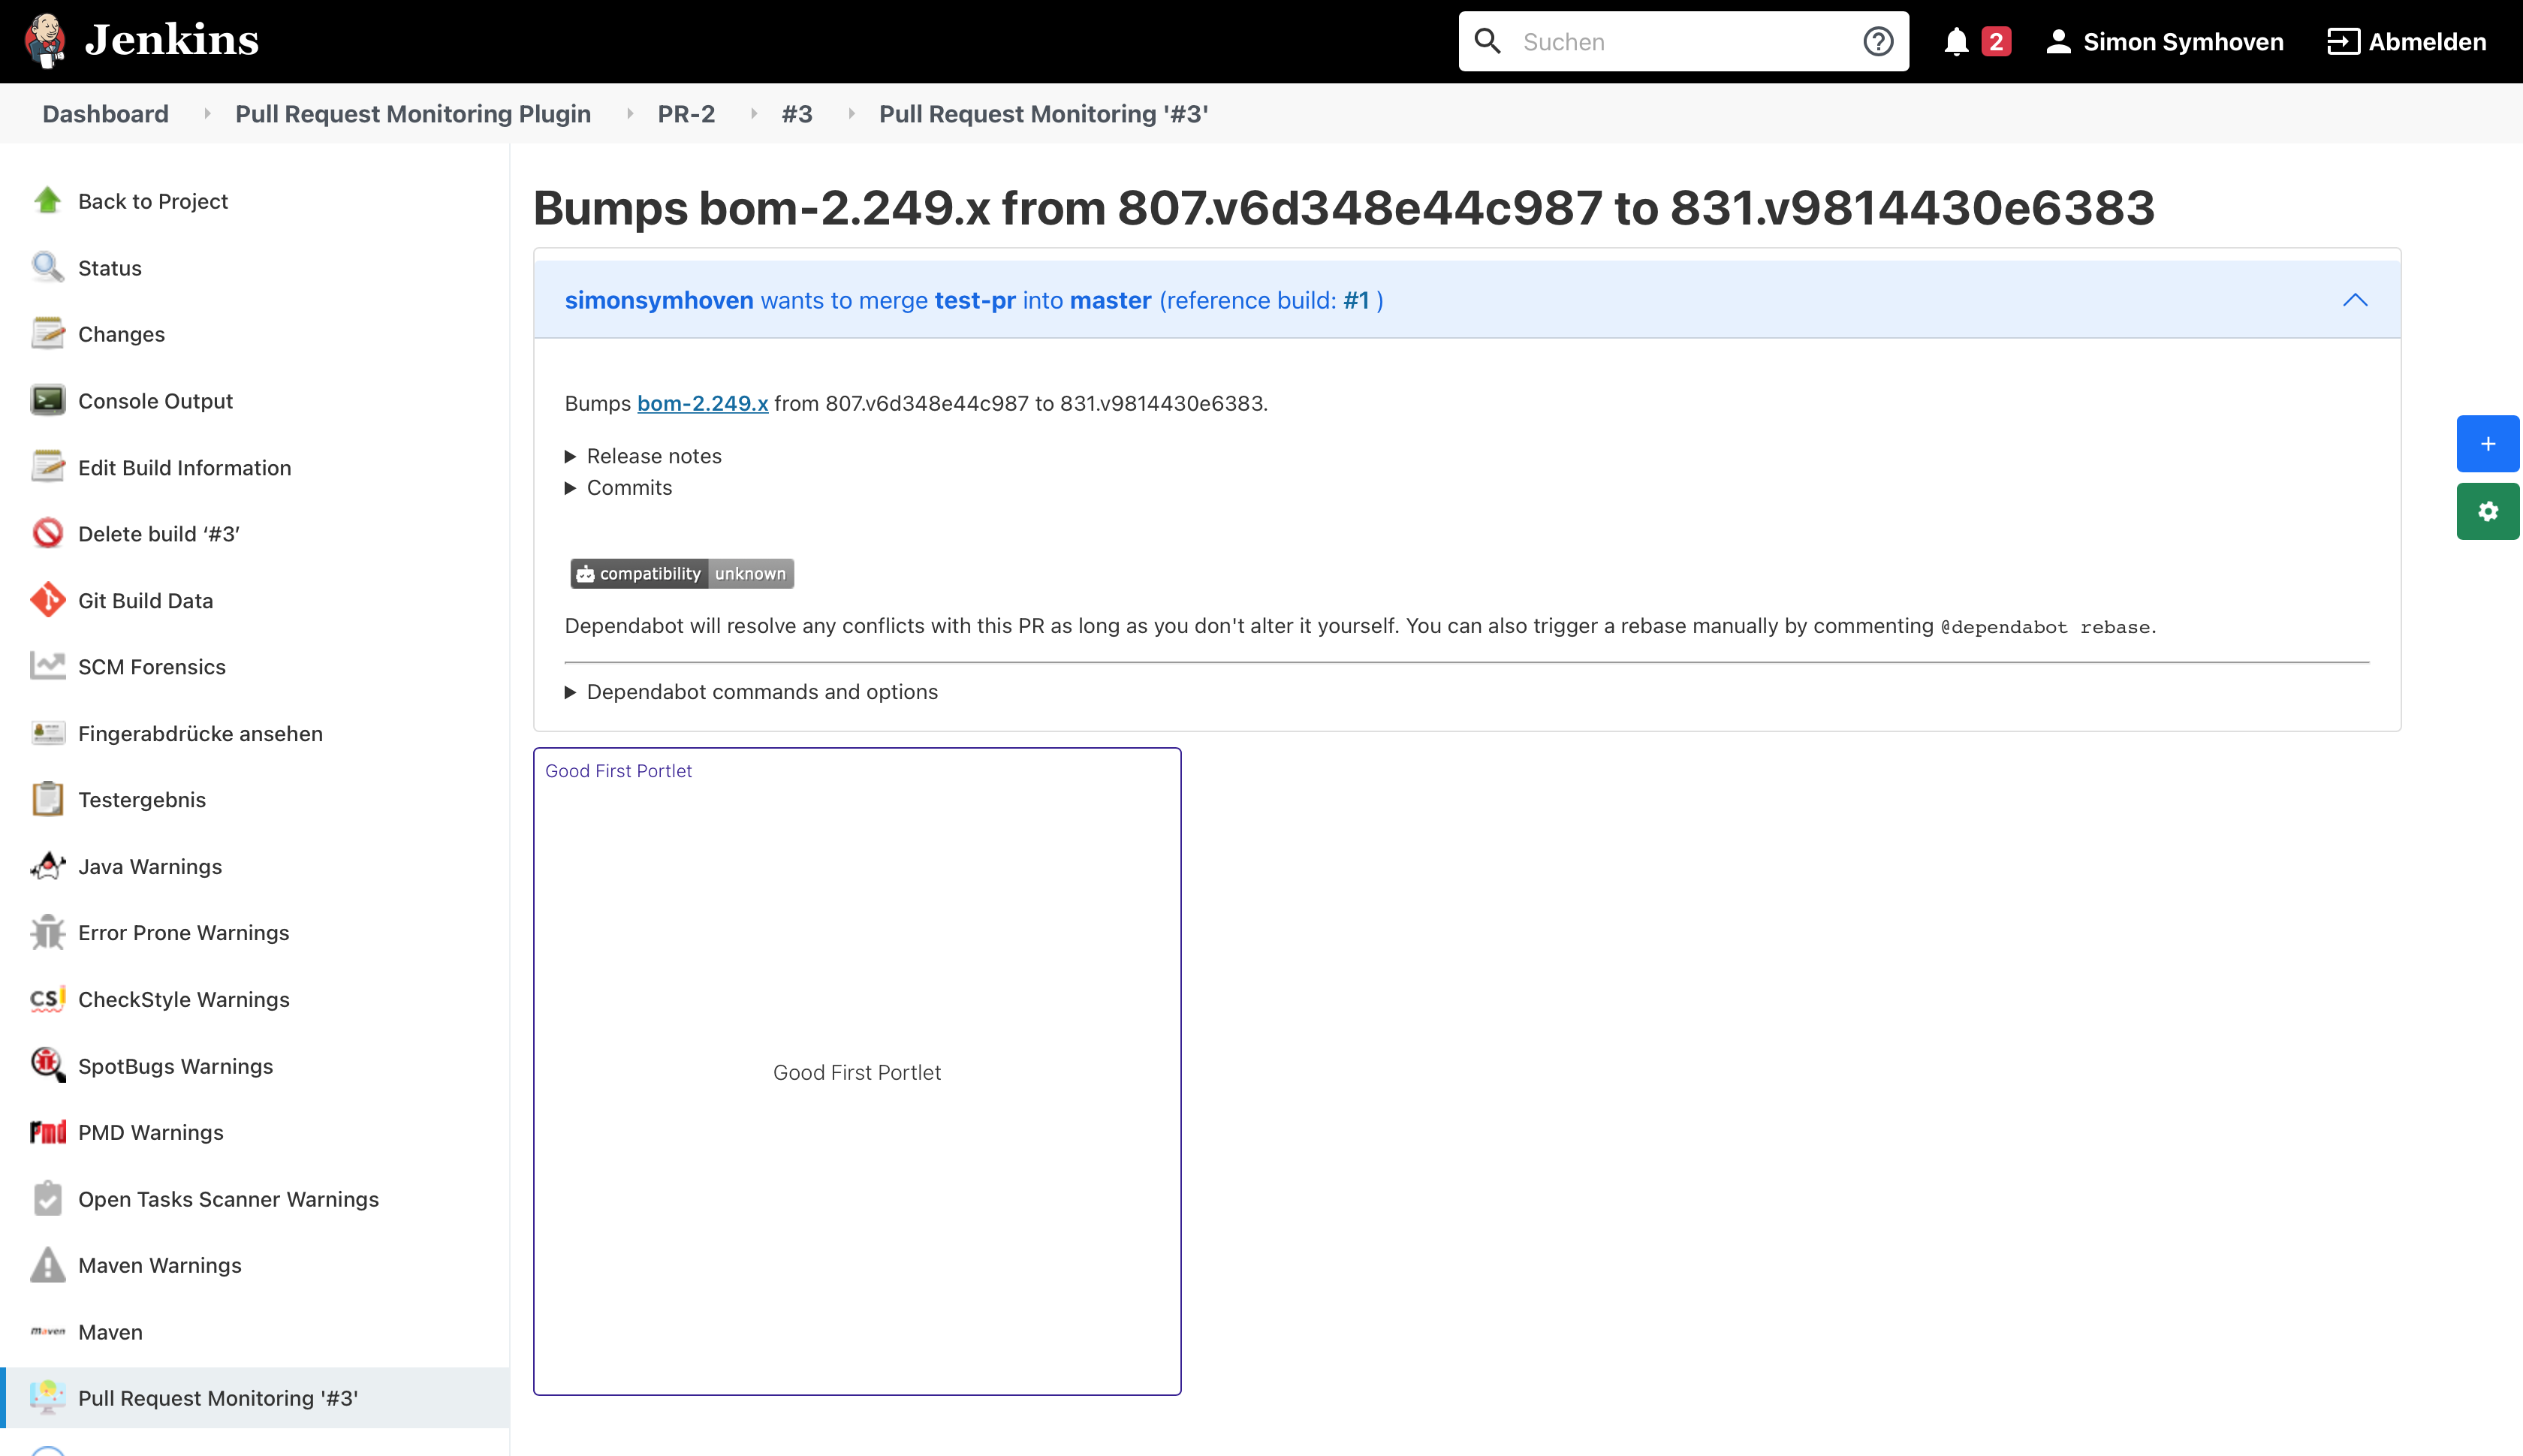
\includegraphics[width=\textwidth]{source/images/metadata}
\caption[Metadaten eines \textit{Pull Requests}.]{Metadaten eines \textit{Pull Requests}, Quelle: Eigene Aufnahme.}
\label{fig:metadata}
\end{figure}

\subsubsection{\textit{Portlets} hinzufügen}
\label{chap:add}

Um ein neues \textit{Portlet} hinzuzufügen, muss zunächst aus der Liste der verfügbaren \textit{Portlets} eines ausgewählt werden, wie \autoref{fig:add1} zeigt. Ist dieses bereits im Layout enthalten, so wird das entsprechende \textit{Portlet} ausgegraut. Falls gewünscht, kann die vordefinierte Breite und Höhe des ausgewählten \textit{Portlets} modifiziert und überschrieben werden. Auch die Farbe kann verändert werden. \autoref{fig:add2} zeigt die Einstellungen für das selektierte \textit{Java} \textit{Portlet} aus dem \textit{Warnings Next Generation Plugin}.

\begin{figure}[h!]
\begin{minipage}[t]{0.49\textwidth}
\centering
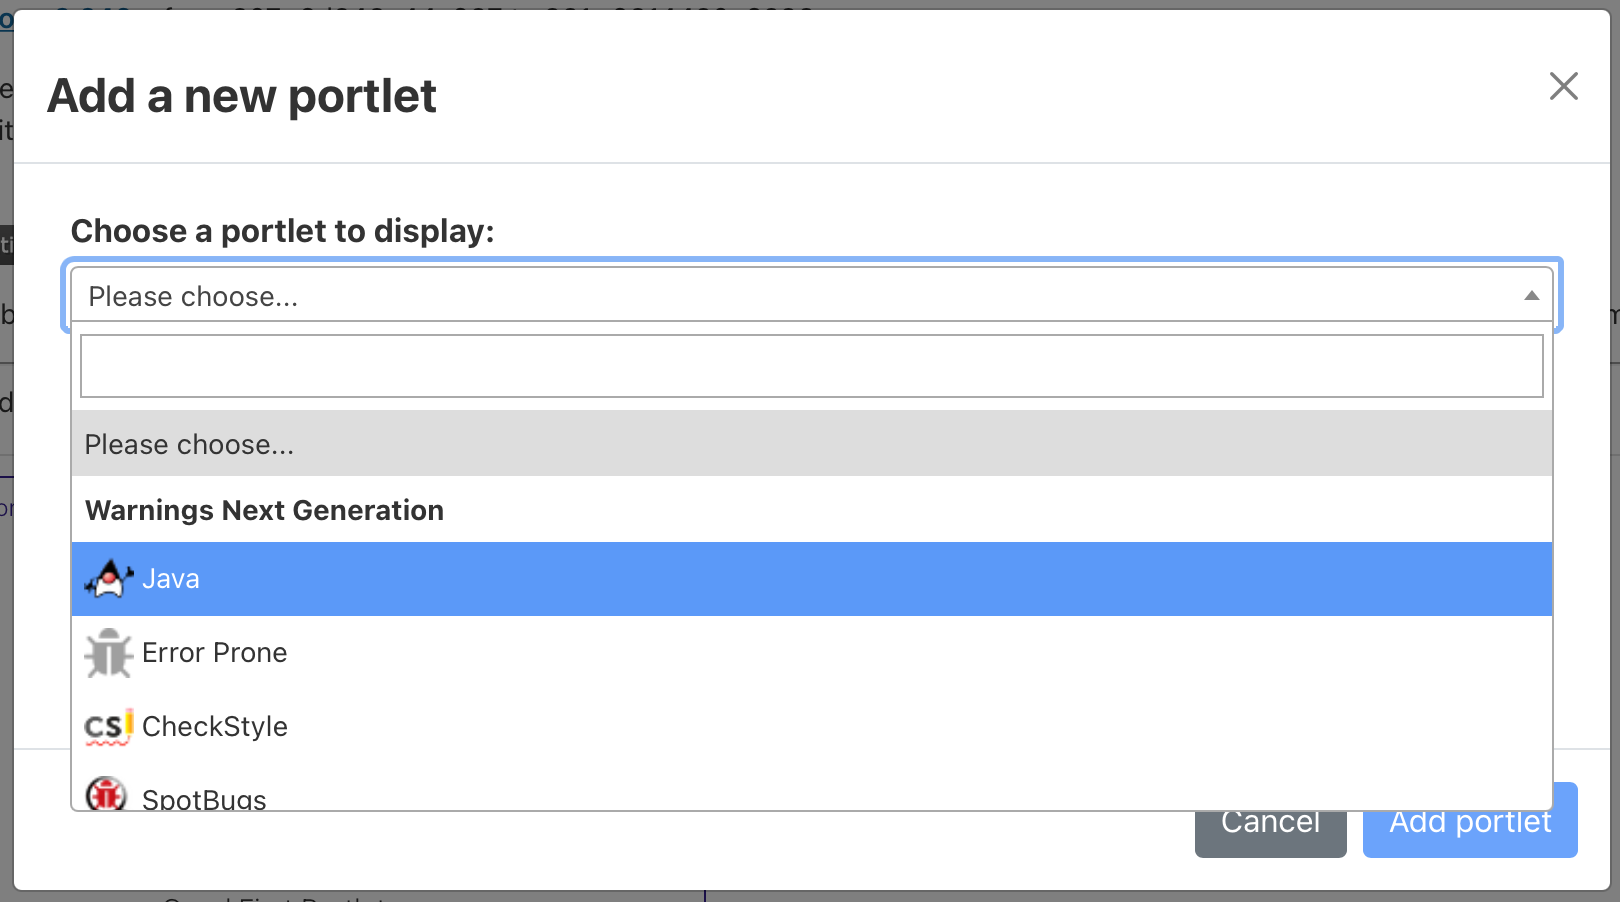
\includegraphics[width=\textwidth]{source/images/add1}
\caption[Ein neues \textit{Portlet} hinzufügen. Auswahl des \textit{Portlets}.]{Ein neues \textit{Portlet} hinzufügen. Auswahl des \textit{Portlets}, Quelle: Eigene Aufnahme.}
\label{fig:add1}
\end{minipage}
\hspace{0.1cm}
\begin{minipage}[t]{0.49\textwidth}
\centering
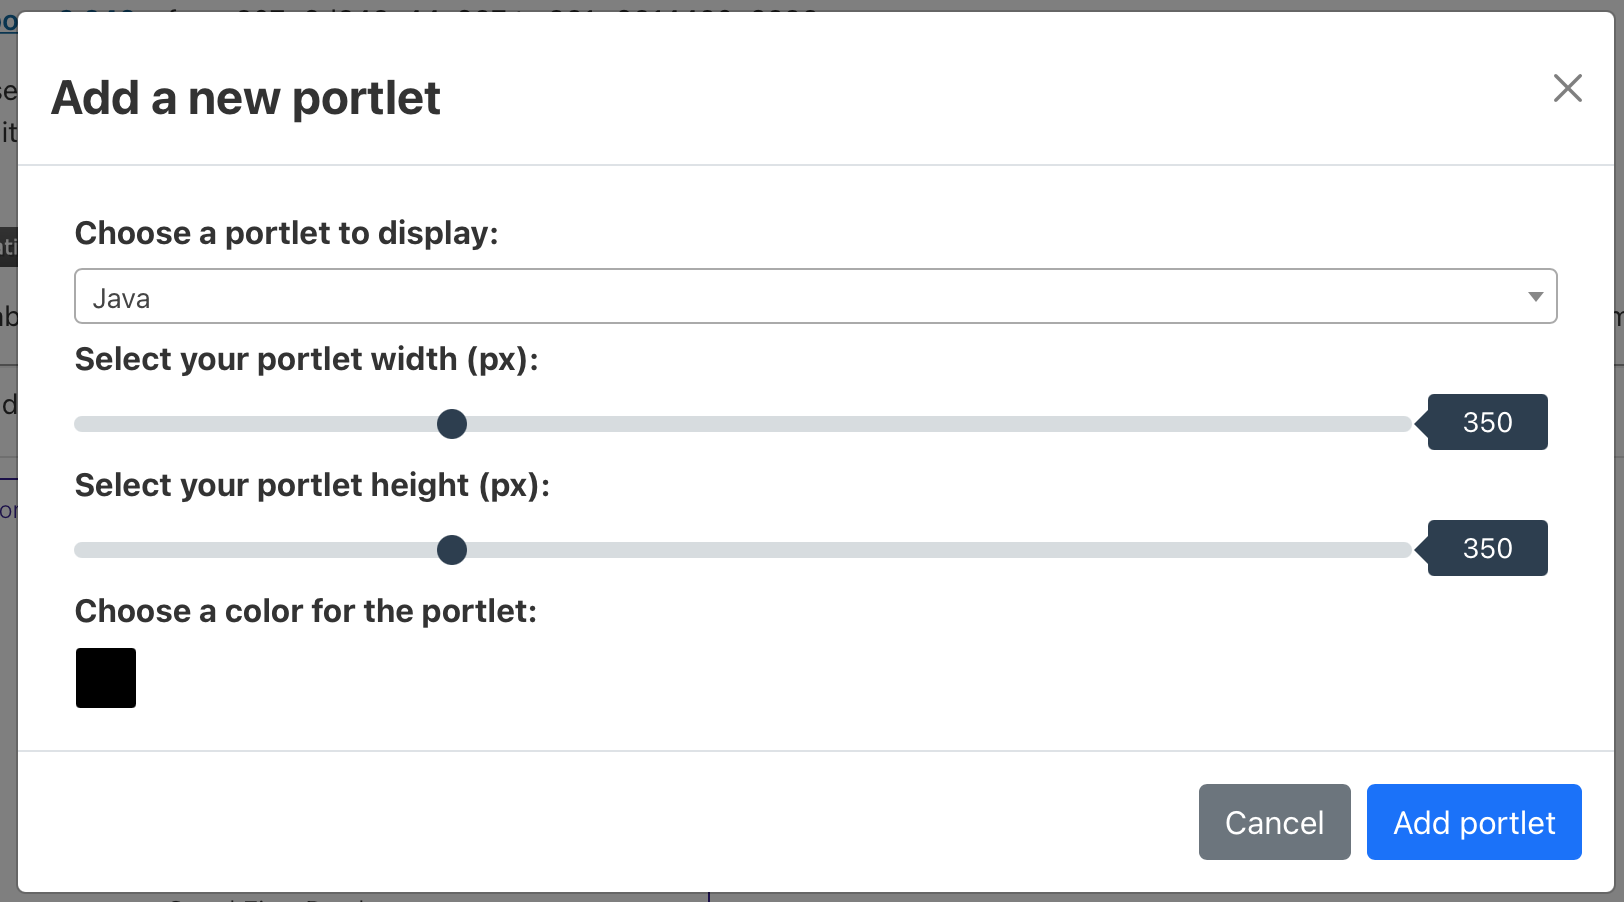
\includegraphics[width=\textwidth]{source/images/add2}
\caption[Ein neues \textit{Portlet} hinzufügen. Auswahl der Größe und Farbe.]{Ein neues \textit{Portlet} hinzufügen. Auswahl der Größe und Farbe, Quelle: Eigene Aufnahme.}
\label{fig:add2}
\end{minipage}
\end{figure}


\subsubsection{Einstellungen}
\label{chap:settings}

Die Einstellungen aus \autoref{fig:settings} bieten dem Nutzer die Möglichkeit, bestimmte Informationen über das Dashboard einzusehen. Es wird ermittelt, ob es Änderungen an der Konfiguration in der \textit{Pipeline} seit dem letzten \textit{Run} gibt und die Quelle der Konfiguration angezeigt. Diese kann entweder \textit{Default} oder \textit{User-Specific} sein. Außerdem wird berechnet, ob die aktuelle Konfiguration mit der \textit{default}-Konfiguration übereinstimmt. Der Anwender hat die Möglichkeit, die aktuelle Konfiguration zu jeder Zeit auf die \textit{default}-Konfiguration zurückzusetzen. Die beiden Konfiguration werden außerdem als \textit{JSON-Tree} mit ihren Attributen abgebildet. 

\begin{figure}[h!]
\centering
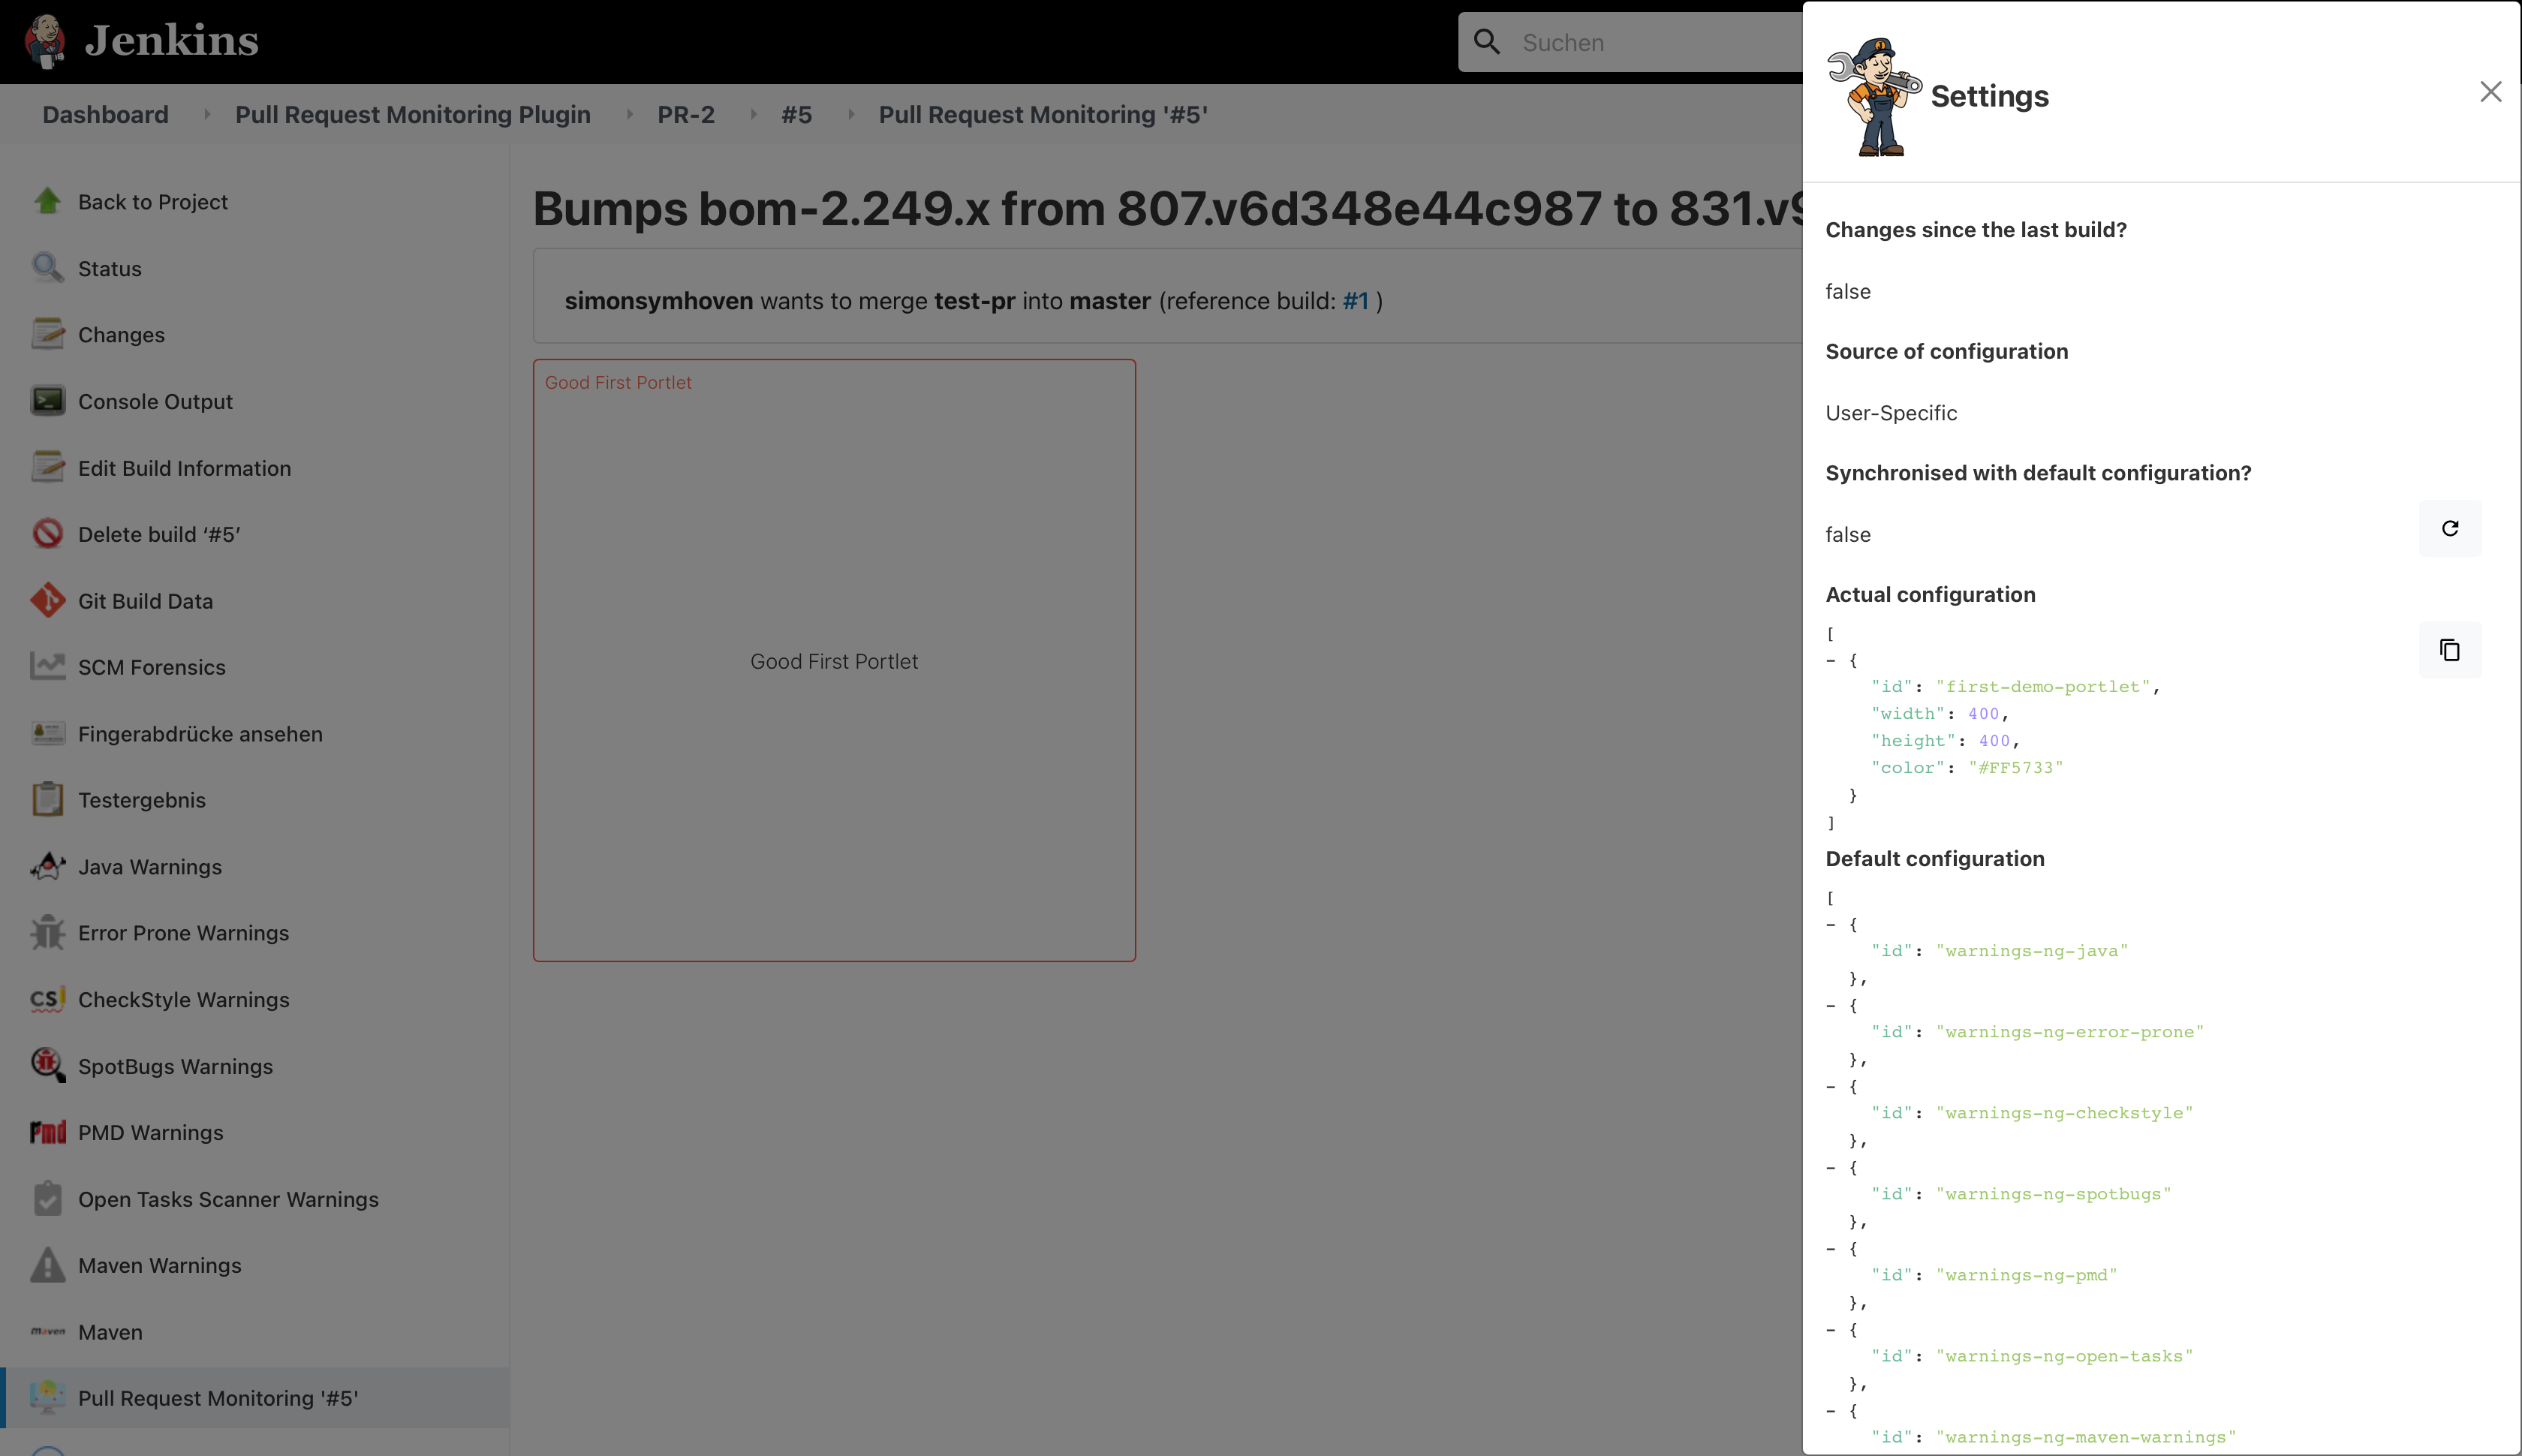
\includegraphics[width=\textwidth]{source/images/settings}
\caption[Ansicht: Einstellungen.]{Ansicht: Einstellungen, Quelle: Eigene Aufnahme.}
\label{fig:settings}
\end{figure}


\section{Verfügbare \textit{Portlets}}

Neben dem \textit{Plugin} selbst wurde während der Entwicklung der vorliegenden Arbeit das entwickelte \ac{api} verwendet, um zwei dieser \textit{Portlets} in anderen \textit{Jenkins} \textit{Plugins} zu entwickeln. So konnte das \ac{api} auf Tauglichkeit geprüft werden und erleichtert das Entwickeln weiterer \textit{Portlets} für andere \textit{Plugin} Betreiber.

\subsection{\textit{Warnings Next Generation Plugin}}
\label{chap:warnings-ng}

\flqq{Das \textit{Warnings Next Generation Plugin} sammelt Compiler-Warnungen oder Probleme, die von statischen Analysewerkzeugen gemeldet werden, und visualisiert die Ergebnisse. Es hat eingebaute Unterstützung für mehr als hundert Berichtsformate.\frqq{}, schreibt \citet{warnings-ng-plugin} über sein \textit{Plugin}. Das \textit{Warnings Next Generation Plugin} liefert für jedes dieser Analysewerkzeuge mithilfe der \textit{MonitorPortletFactory} ein \textit{Portlet} aus. Die grafische Darstellung der Ergebnisse unterscheidet sich von \textit{Portlet} zu \textit{Portlet} nicht - lediglich die zugrundeliegenden Daten ändern sich. Somit wird eine Klasse \textit{MonitorPortlet} verwendet und für jedes Analysewerkzeug eine Instanz dieser Klasse mit den spezifischen Ergebnissen ausgeliefert. Dabei werden drei Fälle unterschieden:

\begin{enumerate}
	\item	Es liegen keine Warnungen vor (\autoref{fig:warning1}).
	\item Es gibt keine neuen Warnungen, aber ausstehende und eventuell gelöste Warnungen (\autoref{fig:warning2}).
	\item Es gibt neue Warnungen. Dazu eventuell ausstehende und gelöste Warnungen (\autoref{fig:warning3}).
\end{enumerate}

\begin{figure}[H]
\begin{minipage}[t]{0.45\textwidth}
\centering
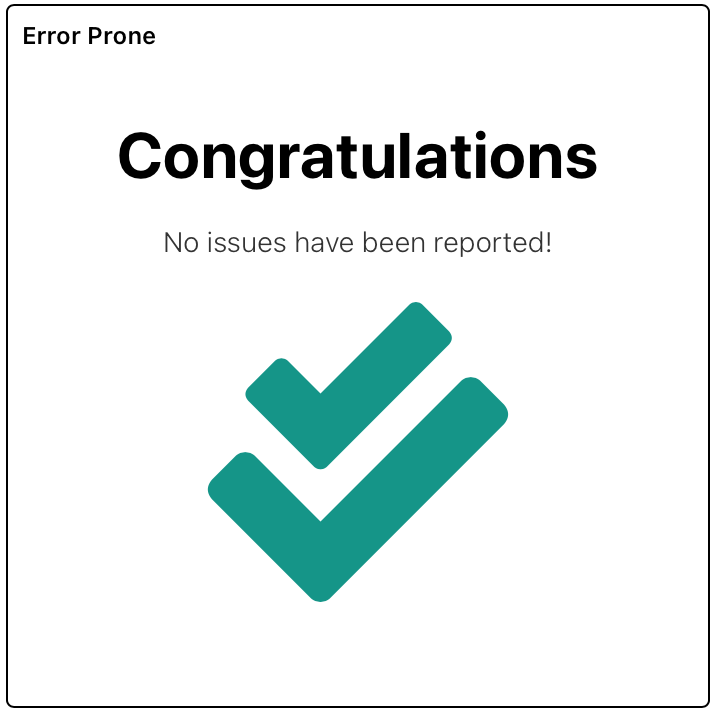
\includegraphics[width=\textwidth]{source/images/warning1}
\caption[\textit{Portlet} des \textit{Warnings Next Generation Plugins} ohne Warnungen.]{\textit{Portlet} des \textit{Warnings Next Generation Plugins} ohne Warnungen, Quelle: Eigene Aufnahme.}
\label{fig:warning1}
\end{minipage}
\hspace{0.5cm}
\begin{minipage}[t]{0.45\textwidth}
\centering
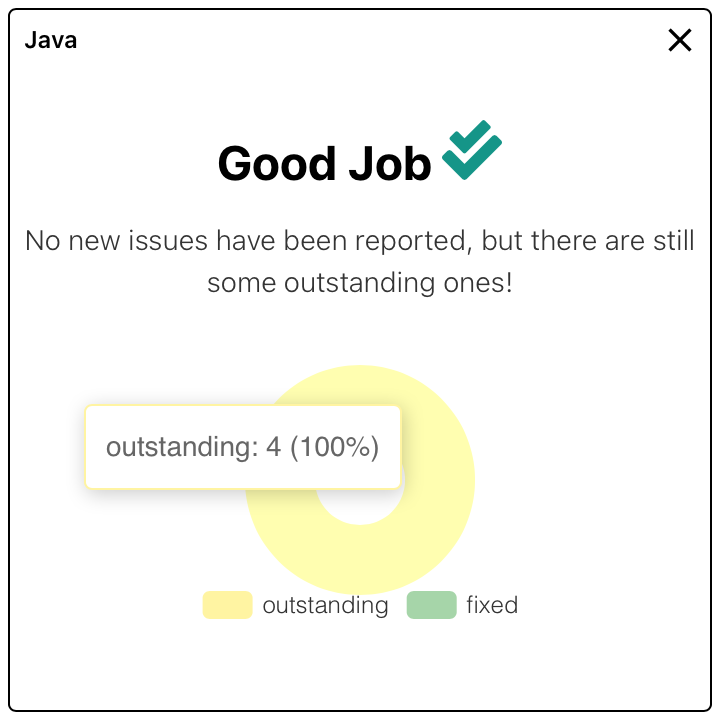
\includegraphics[width=\textwidth]{source/images/warning2}
\caption[\textit{Portlet} des \textit{Warnings Next Generation Plugins} ohne neue Warnungen .]{\textit{Portlet} des \textit{Warnings Next Generation Plugins} ohne neue Warnungen, Quelle: Eigene Aufnahme.}
\label{fig:warning2}
\end{minipage}

\begin{minipage}[t]{0.45\textwidth}
\centering
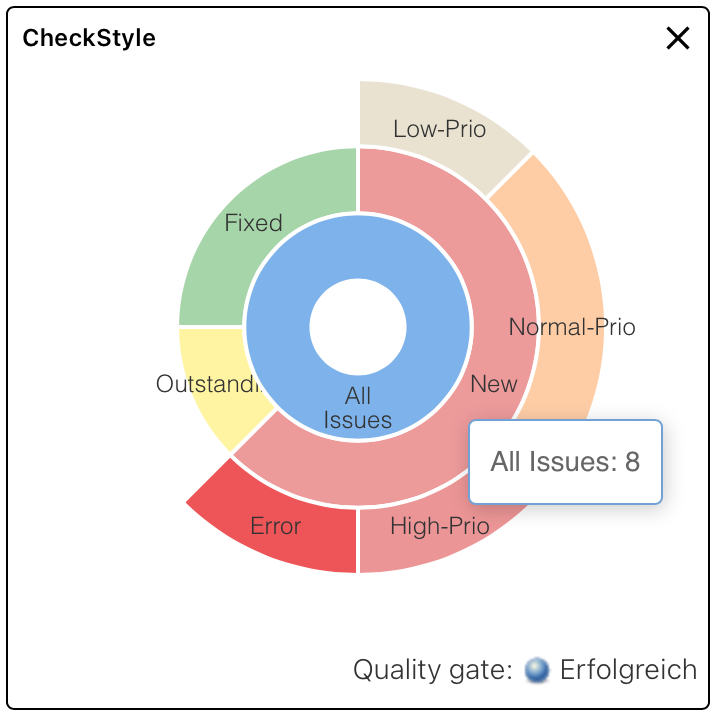
\includegraphics[width=\textwidth]{source/images/warning3}
\caption[\textit{Portlet} des \textit{Warnings Next Generation Plugins} mit Warnungen.]{\textit{Portlet} des \textit{Warnings Next Generation Plugins} mit Warnungen, Quelle: Eigene Aufnahme.}
\label{fig:warning3}
\end{minipage}
\end{figure}

\subsection{\textit{Code Coverage API Plugin}}
\label{chap:code-coverage-api}

Das \textit{Code Coverage API Plugin} dient als \ac{api} zur Integration und Veröffentlichung mehrerer \textit{Coverage Reports} \citep{code-coverage-api-plugin}. Das \textit{Portlet} visualisiert die \textit{Conditional}- und \textit{Line}-\textit{Coverage} bezogen auf den aktuellen \textit{Run} und erzeugt aus den Metriken ein Balkendiagramm. Zusätzlich wird die Differenz zu dem Referenz-\textit{Run} kalkuliert und als Delta hinter der jeweiligen \textit{Coverage} ausgegeben. Die absolute \textit{Conditional}- und \textit{Line}-\textit{Coverage} aus dem \textit{Run} beträgt 78,57 \% bzw. 81,82 \%. Die Delta-\textit{Coverage} bezogen auf den Referenz-\textit{Run} des Ziel-\textit{Branches} hat sich nicht verändert. Die \textit{Code Coverage} (\textit{Conditional} und \textit{Line}) ist folglich in Quell- und Ziel-\textit{Branch} dieselbe und wird durch den \textit{Pull Request} nicht vermindert oder verbessert.

\begin{figure}[H]
\centering
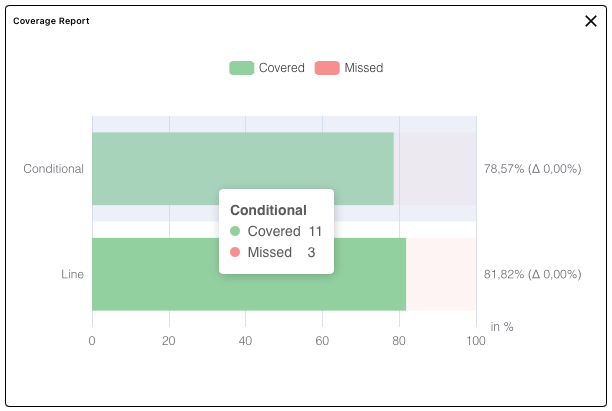
\includegraphics[width=\textwidth]{source/images/coverage}
\caption[\textit{Portlet} des \textit{Code Coverage API Plugins}.]{\textit{Portlet} des \textit{Code Coverage API Plugins}, Quelle: Eigene Aufnahme.}
\label{fig:coverage}
\end{figure}

\chapter{Diskussionen}
\label{chap:diskussionen}

\section{Allgemeine Voraussetzung}
Kernaufgabe des \textit{Jenkins \ac{ci}}-Servers ist die  Ausführungen von \textit{Jobs}. Es gibt \textit{Freestyle-Jobs}, in denen die einzelnen \textit{Build Steps} konfigurierbar definiert werden. \textit{Pipelines} sind spezielle \textit{Jobs}, deren Definition in Form von \textit{Groovy}-Code erfolgt. Diese können in der \textit{Job}-Konfiguration oder im \ac{scm} abgelegt werden. Durch die Ablage im \ac{scm} und der Verwendung des \textit{Plugins} \textit{Pipeline: Mutlibranch} wird das Erkennen von verschiedenen \textit{Branches} in dem verwendeten \ac{scm}-\textit{Repository} ermöglicht. Jeder \textit{Branch} wird als ein separater \textit{Job} behandelt, für den unabhängige Arbeitsabläufe als \textit{Pipeline} oder innerhalb der \textit{Job} Konfiguration definiert werden können \citep{workflow-multibranch-plugin}. 
Das \textit{Pull Request Monitoring Plugin} beschränkt sich auf die Verwendung von \textit{Multibranch} Projekten. 


\section{\textit{Abstract Class} statt \textit{Interface}}
Mit Version \textit{1.6.0} wurden die beiden Klassen \textit{MonitorPortlet} und \textit{MonitorPortletFactory} von einem \textit{Interface} zu einer \textit{Abstract Class} geändert \citep{pull-request-monitoring-plugin}. Dies bietet den Vorteil, dass bestimmte Methoden mit einer Implementierung belegt werden können, die nur bei Bedarf von der erbenden Klasse überschrieben werden müssen. Des Weiteren bietet die Verwendung einer \textit{Abstract Class} eine deutlich stabilere Schnittstelle nach außen an, da im Falle von einer Erweiterung eine vordefinierte Implementierung der hinzugefügten Methode mitgeliefert werden kann, sodass es bei der erbenden Klasse zu keinen Fehlern während des Kompilierens kommt.

\section{\textit{User Property} statt \textit{Local Storage}}

Bis Version \textit{1.0.3-beta} wurde die Konfiguration des \textit{Dashboards}, also der im \textit{Dashboard} verwendeten \textit{Portlets} im lokalen Speicher, dem \textit{Local Storage} des Browsers persistiert. Darunter die Breite, Höhe und die eindeutige ID jedes \textit{Portlets}, um diese beispielsweise bei der Aktualisierung der Seite erneut zu laden \citep{pull-request-monitoring-plugin}. Diese erste lauffähige Beta-Version wurde im \textit{Jenkins UX SIG Meeting}, dem \textit{Jenkins User Experience Special Interest Group Meeting} präsentiert \citep{yt}. Tim Jacomb, ein aktives Mitglied der \textit{UX SIG} Gruppe, merkte an, dass das Speichern der Konfiguration im lokalen Speicher des Browsers diverse Nachteile mit sich bringt. Konfigurationen sind somit abhängig vom eingesetzten Browser, können also beim Verwenden eines anderen Browsers nicht übernommen werden. Dasselbe gilt, wenn Nutzer sich an unterschiedlichen Rechnern anmelden, um auf eine \textit{Jenkins} Instanz zuzugreifen. Er schlug vor die Konfiguration stattdessen in einer \textit{User Property}, der \textit{MonitorConfigurationProperty} innerhalb der \textit{Jenkins} Infrastruktur zu speichern, um zu jederzeit browser- und rechnerunabhängig auf die Konfiguration zugreifen zu können. 
 
\section{Auswahl der \textit{JavaScript} Bibliothek \textit{Muuri}}

Es existieren diverse \textit{JavaScript} Bibliotheken, welche bereits ein konfigurierbares, verschiebbares und dynamisches Layout für ein \textit{Dashboard} zur Verfügung stellen, darunter \textit{gridstack.js} \citep{gridstack} oder \textit{Muuri}. \textit{Muuri} stellte sich als für diesen Zweck einzig brauchbare Bibliothek heraus, da es diese dem Entwickler erlaubt, den Inhalt der einzelnen \textit{Items}, den \textit{Portlets} als HTML zu setzen und über Klassenzuweisungen dem \textit{Dashboard} hinzuzufügen und zu steuern.
Bei \textit{gridstack.js} ist dies nicht möglich. Hier muss der zu setzende Inhalt statisch über das \textit{API} der Bibliothek gesetzt werden. Das stellte sich als nicht praktikabel heraus, da die bereitgestellten \textit{Portlets} als \textit{Jelly-View} ausgeliefert werden. Diese können nur in anderen \textit{Jelly-Views} inkludiert werden und nicht im Nachhinein hinzugefügt werden, da das \textit{Jelly} Rendering serverseitig beim Aufruf der entsprechenden \ac{url} initiiert wird.

\section{\textit{Default}-\textit{Portlets} für das \textit{Dashboard}}
\label{chap:default}

Seit Version 1.7.0 kann ein \textit{Portlet} entscheiden, ob dieses standardmäßig im \textit{Dashboard} angezeigt werden soll \citep{pull-request-monitoring-plugin}. Sofern für das jeweilige \textit{Dashboard} keine nutzerspezifische Konfiguration existiert, werden dem Nutzer beim Öffnen eines zu einem \textit{Run} zugehörigen \textit{Dashboards} alle vorhanden \textit{Portlets} angezeigt, die als \textit{default} markiert sind. Das soll dem Nutzer den Einstieg erleichtern und die manuelle Konfiguration der \textit{Dashboards} vermeiden. Durch lokale Änderungen über das \ac{ui} des \textit{Dashboards} oder die Anwendung einer im \textit{Jenkinsfile} definierten Konfiguration, wird diese \textit{default}-Konfiguration überschrieben. 

\chapter{Zusammenfassung und Ausblick}
\label{chap:fazit}

Statt die Resultate für das Gesamtprojekt zu visualisieren, ist eine gefilterte Darstellung der Ergebnisse auf die tatsächlich vorgenommene Änderung an der Codebasis innerhalb eines \textit{Pull Requests} sinnvoll. Diese Arbeit beschäftigte sich mit der Konzeptionierung und Entwicklung eines \textit{Jenkins} \textit{Plugins} zur Überwachung bestimmter Qualitätskriterien und Metriken eines \textit{Pull Requests}. Diese beziehen sich auf die durch den \textit{Pull Request} veränderte Codebasis - das Delta zwischen Quell- und Ziel-\textit{Branch}. Das Monitoringsystem wird dem Nutzer in Form eines konfigurierbaren und eines durch andere \textit{Plugins} erweiterbaren \textit{Dashboards} innerhalb des \textit{Jenkins} \ac{ui} zur Verfügung gestellt. Die grundlegenden Funktionen des \textit{Dashboards} basieren dabei auf der externen Bibliothek \textit{Muuri}. Die Konfiguration des \textit{Dashboards} wird browser- und rechnerunabhängig pro Nutzer innerhalb des \textit{Jenkins} gespeichert und ist jederzeit abrufbar. Außerdem wurde ein \ac{api} entwickelt, welches andere \textit{Plugins} konsumieren und ihre Metriken als \textit{Portlets} dem Nutzer bereitstellen können. Diese können somit in dem nutzerspezifischen \textit{Dashboard} hinzugefügt und überwacht werden. Dieses \ac{api} wurde im Rahmen der vorliegenden Arbeit verwendet, um die ersten \textit{Portlets} in dem \textit{Warnings Next Generation} und \textit{Code Coverage \ac{api} Plugin} zu entwickeln und zu veröffentlichen. Das \textit{Pull Request Monitoring Plugin} ist unter der \textit{MIT}-Lizenz als \textit{Open Source} Projekt veröffentlicht und 
steht zur Installation innerhalb des \textit{Jenkins} Servers bereit. 

Abschließend werden diejenigen Punkte angesprochen, für die die Zeit nicht ausgereicht hat, die aber im Rahmen weiterer Studien oder Erweiterungen des \textit{Plugins} interessant wären zu untersuchen und umzusetzen.

Die Größe eines \textit{Portlets} wird in Pixeln von dem implementierenden \textit{Plugin} festgelegt und verändert diese Größe nicht, wenn das \textit{Dashboard}, respektive das Browserfenster verkleinert oder vergrößert wird. Denkbar ist es, dies durch ein \textit{Grid}-System zu ersetzen, sodass die Größe der \textit{Portlets} sich der Größe des Browserfensters anpassen, statt eine statische Größe zu definieren.

Des Weiteren können die \textit{Portlets} innerhalb des \textit{Dashboards} nicht bearbeitet werden. Dazu müssen diese zuerst entfernt werden und dann über den Dialog aus \autoref{fig:add2} mit den neuen Parametern dem \textit{Dashboard} wieder hinzugefügt werden. Praktikabler wäre eine Möglichkeit für den Nutzer, die bereits existierenden \textit{Portlets} über einen weiteren Dialog direkt bearbeiten zu können ohne diese vorher löschen zu müssen. 

Ebenfalls sollen für weitere \textit{Plugins} wie dem \textit{JUnit} \citep{junit-plugin} oder dem \textit{Git Forensics} \textit{Plugin} \citep{git-forensics-plugin} \textit{Portlets} entwickelt werden und weitere Autoren motiviert werden, die zur Verfügung gestellte \ac{api}  zu nutzen, um der \textit{Jenkins Community} ein vielfältigeres \textit{Dashboard} bereitstellen zu können. 

Durch die Vorstellung der ersten Beta-Version des \textit{Plugins} in einem der \textit{Jenkins UX SIG} Treffen, wurde die Comquent GmbH aus Puchheim auf das \textit{Plugin} und diese Arbeit aufmerksam.  Dadurch ergab sich die Möglichkeit, die vorliegende Arbeit auch im Kontext der wirtschaftlichen Anwendung zu diskutieren und voraussichtlich in aktiven Projekten bei Kunden der Comquent GmbH einzusetzen. Dadurch wäre es besonders interessant herauszufinden, welche Anforderungen sich aus der wirtschaftlichen Anwendung ergeben, um diese mit in die Weiterentwicklung des \textit{Plugins} einfließen lassen zu können. In einem ersten Gespräch mit dem Geschäftsführer der Comquent GmbH, Herrn Andreas Schönfeld, wies dieser darauf hin, dass sich die Anforderungen der Wirtschaft nicht selten von denen aus der Entwickler-Szene unterscheiden, da Trends, Prozesse und Arbeitsweisen häufig sehr viel später antizipiert werden. 
Als mögliche Weiterentwicklung des \textit{Plugins} wurden die Einflussfaktoren der Delta-Resultate diskutiert: Welcher Entwickler hat durch welche Änderungen welche Metriken wie verändert? 
Aufgrund der zeitlichen Einschränkungen können die Ergebnisse der praktischen Anwendung nicht in der vorliegenden Arbeit diskutiert werden. 
Besonders bedanke ich mich bei Herrn Andreas Schönfeld für die Kooperation und die Zusammenarbeit. Diese hat mir wertvolle Einblicke gewährt und eine praxisnahe Forschung ermöglicht, die über diese Arbeit hinaus anhalten wird.

%Einbinden der Verzeichnisse
\backmatter

%Liste der Tabellenverzeichnisses
\listoftables
\addcontentsline{toc}{chapter}{Tabellenverzeichnis}

%Einbinden des Abbildungsverzeichnisses
\listoffigures
\addcontentsline{toc}{chapter}{Abbildungsverzeichnis}

%Einbinden des Sourcecodeverzeichnisses
\lstlistoflistings
\addcontentsline{toc}{chapter}{Listings}

% Quellenverzeichnis
\phantomsection
\addcontentsline{toc}{chapter}{Literaturverzeichnis}
\appendix
\bibliographystyle{dinat}
\bibliography{source/bib/references.bib}

% Anhang
%\appendix
%\include{source/content/Danksagung}
\end{document}
